%%
%% This is file `sample-sigconf.tex',
%% generated with the docstrip utility.
%%
%% The original source files were:
%%
%% samples.dtx  (with options: `sigconf')
%% 
%% IMPORTANT NOTICE:
%% 
%% For the copyright see the source file.
%% 
%% Any modified versions of this file must be renamed
%% with new filenames distinct from sample-sigconf.tex.
%% 
%% For distribution of the original source see the terms
%% for copying and modification in the file samples.dtx.
%% 
%% This generated file may be distributed as long as the
%% original source files, as listed above, are part of the
%% same distribution. (The sources need not necessarily be
%% in the same archive or directory.)
%%
%% Commands for TeXCount
%TC:macro \cite [option:text,text]
%TC:macro \citep [option:text,text]
%TC:macro \citet [option:text,text]
%TC:envir table 0 1
%TC:envir table* 0 1
%TC:envir tabular [ignore] word
%TC:envir displaymath 0 word
%TC:envir math 0 word
%TC:envir comment 0 0
%%
%%
%% The first command in your LaTeX source must be the \documentclass command.

%\documentclass[sigconf]{acmart}
\documentclass[sigconf,screen,nonacm]{acmart}

%% NOTE that a single column version may be required for 
%% submission and peer review. This can be done by changing
%% the \doucmentclass[...]{acmart} in this template to 
%% \documentclass[manuscript,screen]{acmart}
%% 
%% To ensure 100% compatibility, please check the white list of
%% approved LaTeX packages to be used with the Master Article Template at
%% https://www.acm.org/publications/taps/whitelist-of-latex-packages 
%% before creating your document. The white list page provides 
%% information on how to submit additional LaTeX packages for 
%% review and adoption.
%% Fonts used in the template cannot be substituted; margin 
%% adjustments are not allowed.
%%
%%
%% \BibTeX command to typeset BibTeX logo in the docs
\AtBeginDocument{%
  \providecommand\BibTeX{{%
    \normalfont B\kern-0.5em{\scshape i\kern-0.25em b}\kern-0.8em\TeX}}}

%% Rights management information.  This information is sent to you
%% when you complete the rights form.  These commands have SAMPLE
%% values in them; it is your responsibility as an author to replace
%% the commands and values with those provided to you when you
%% complete the rights form.
\setcopyright{acmlicensed}
\copyrightyear{2024}
\acmYear{2024}

%% These commands are for a PROCEEDINGS abstract or paper.
\acmConference[University of Colorado]{CSPB 4502 - Data Mining}{March 18,
  2024}{Boulder, CO}
%
%  Uncomment \acmBooktitle if th title of the proceedings is different
%  from ``Proceedings of ...''!
%
%\acmBooktitle{Woodstock '18: ACM Symposium on Neural Gaze Detection,
%  June 03--05, 2018, Woodstock, NY} 
\acmISBN{978-1-4503-XXXX-X/18/06}


%%
%% Submission ID.
%% Use this when submitting an article to a sponsored event. You'll
%% receive a unique submission ID from the organizers
%% of the event, and this ID should be used as the parameter to this command.
%%\acmSubmissionID{123-A56-BU3}

%%
%% For managing citations, it is recommended to use bibliography
%% files in BibTeX format.
%%
%% You can then either use BibTeX with the ACM-Reference-Format style,
%% or BibLaTeX with the acmnumeric or acmauthoryear sytles, that include
%% support for advanced citation of software artefact from the
%% biblatex-software package, also separately available on CTAN.
%%
%% Look at the sample-*-biblatex.tex files for templates showcasing
%% the biblatex styles.
%%

%%
%% The majority of ACM publications use numbered citations and
%% references.  The command \citestyle{authoryear} switches to the
%% "author year" style.
%%
%% If you are preparing content for an event
%% sponsored by ACM SIGGRAPH, you must use the "author year" style of
%% citations and references.
%% Uncommenting
%% the next command will enable that style.
%%\citestyle{acmauthoryear}

%%
%% end of the preamble, start of the body of the document source.
\begin{document}
\pagestyle{fancy}
%\fancyhf{} % Clear all header and footer fields
\fancyfoot[C]{\thepage} % Center the page number in the footer
%\thispagestyle{fancy} % Apply the fancy page style to the first page as well

%%
%% The "title" command has an optional parameter,
%% allowing the author to define a "short title" to be used in page headers.
\title{COVID-19 Comprehensive Study}

%%
%% The "author" command and its associated commands are used to define
%% the authors and their affiliations.
%% Of note is the shared affiliation of the first two authors, and the
%% "authornote" and "authornotemark" commands
%% used to denote shared contribution to the research.
\author{Mohammed Alsailani}
\authornote{All authors contributed equally to this research.}
\affiliation{%
  \institution{University of Colorado Boulder}
}

\author{Andrew Byrnes}
\authornotemark[1]
\affiliation{%
  \institution{University of Colorado Boulder}
}

\author{Collin Coakley}
\authornotemark[1]
\affiliation{%
  \institution{University of Colorado Boulder}
}


\author{Gilberto Zamarron}
\authornotemark[1]
\affiliation{%
  \institution{University of Colorado Boulder}
}

%%
%% By default, the full list of authors will be used in the page
%% headers. Often, this list is too long, and will overlap
%% other information printed in the page headers. This command allows
%% the author to define a more concise list
%% of authors' names for this purpose.
\renewcommand{\shortauthors}{Alsailani et al. 2024}

%%
%% The abstract is a short summary of the work to be presented in the
%% article.

%%
%% The code below is generated by the tool at http://dl.acm.org/ccs.cfm.
%% Please copy and paste the code instead of the example below.
%%


%%
%% Keywords. The author(s) should pick words that accurately describe
%% the work being presented. Separate the keywords with commas.
%\keywords{COVID-19, Data Mining}

%% A "teaser" image appears between the author and affiliation
%% information and the body of the document, and typically spans the
%% page.


\received{22 April 2024}
%\received[revised]{18 Match 2024}
%\received[accepted]{18 Match 2024}

%%
%% This command processes the author and affiliation and title
%% information and builds the first part of the formatted document.
\maketitle

\section{Introduction}
Our project focuses on analyzing data related to COVID-19, including the effect of vaccination on transmission and death. We also look at other local variables, such as temperature, humidity, and population density to track the spread of the virus. Our analysis also use geospatial analysis to look for hot spots and infection surges to see how surrounding counties are impacted. We are relying on the \href{https://health.google.com/covid-19/open-data/}{COVID-19 Open Data by Google}, which provides differing levels of granularity to allow us to focus on different analyses, providing data from 1/1/2020 to 9/17/2022 of various scopes, from world-wide aggregate data, to data about individual counties in any given state in the US. This data was compiled by researchers who authored a paper called \textit{COVID-19 Open-Data a global-scale spatially granular meta-dataset for coronavirus disease} \cite{wahltinez2022covid}.\\ \\
Our motivation is multifaceted. First, COVID-19 is a unique event in our lifetime that impacted the world in an unprecedented way. The urgency of finding a solution to the pandemic resulted in a large amount of data being collected, making it a good topic for a data mining project. 
\cite{wahltinez2022covid}. \\

The intriguing questions we aim to answer are:  
\begin{itemize}
    \item How are COVID rates correlated with local variables such as: \begin{enumerate}
        \item Temperature % maybe use a 2 week moving avg of temp & 1-week new COVID cases
        \item Humidity % maybe 2 week moving avg
        \item Population density %maybe , affect COVID rates? 
        \item Mobility metrics
        \item rain fall % Are older individuals more susceptible to mortality?
    \end{enumerate}
    \item Classification of counties or general areas COVID-19 hotpots using geospatial analysis
        \begin{enumerate} 
            \item potential classification of areas as hot spots or areas experiencing a surge in infections
            \item The effect of a surge on surrounding areas, including an attempt to analyze factors, such as mobility, that make an area more or less resistant to a surge in cases when nearby area(s) is experiencing a surge.
        \end{enumerate}

    \item Did high vaccination rates help mitigate the deaths and spread of the virus?

    \item Understand the impact of detailed weather variables on COVID-19 rates.
    \end{itemize}

    
% Interesting questions

%comment block
\begin{comment}
This is a commented-out section using the comment package.
None of the text within the \begin{comment} ... \end{comment} block will be processed by LaTeX.
\end{comment}

\section{Related Work}
A broad range of prior work has been performed on this data due to the significant global impact of COVID-19 on society over the past four years. These data have been applied to economic impact analysis, public health policy analysis, modeling virus spread, assessment of success and failure of containment measures, health and healthcare impact forecasts, and more. This dataset has informed researchers, scientists, and healthcare workers in numerous facets of their efforts to effectively allocate resources for vaccine distribution and information dissemination to combat the spread of COVID-19. Fuchs, A. et al \cite{fuchs2020mask} used the dataset to analyse China’s exports of medical goods in times of COVID-19. Arpino, B., et al \cite{arpino2020no} used the data to show that available evidence on the link between intergenerational relationships and COVID-19 is inconclusive. While Murrell, H. et al. \cite{murrell2020estimating} used the data to estimate Rt from Covid-19 data, using SIR models. Studying how infection or vaccination triggers both cellular and humoral responses is essential to know the grade and length of protection generated in the population.

The profound impact of COVID-19 on the world occurred during an era characterized by widespread access to information, leading to extensive research efforts due to its global significance. As a result, many of the data analysis techniques utilized in our study have already been used to some extents in previous research papers. Despite the similarities in techniques used in previous literature, our dataset appears to have been underutilized in comparison. As a result, there may be differences between our findings and those of other studies, or it is possible that we have independently arrived at similar conclusions through our own analyses.

\section{Data set}
The COVID-19 Open Data can be downloaded as world-wide aggregate data, but the data for some countries was sparse in comparison to the US data by county, which was more reliably reported in this dataset. As such, while we plan to clean our data to account for missing values or sparse data, we believe a stronger foundation in the US data by county presents a better baseline dataset for purposes of data mining in this class. As such, we downloaded each US state by county, for a total of 3,228 CSV files with 991 rows of data each on average, and we are storing that in our \href{https://github.com/CCoakley6/DataMiningProjectSpring2024}{group GitHub}. COVID-19 Open Data is most comprehensive COVID-19 dataset we are aware of. It contains collection of epidemiological metrics, including cases, deaths, recoveries, and tests, with variability in data availability across different regions. It highlights the differentiation between new and cumulative data to accommodate adjustments in counting criteria and corrections.

\section{Main Techniques Applied}

\subsection{Preprocessing}

\begin{comment}
    - classification: hot spots/zones for mortality, infection, death
    - geographical analysis: (need to pull in geospatial data) of the spread (potentially from areas identified as hot spots or areas that had recent high infection)
    - correlation: between temperature, humidity, etc
\end{comment}

\textbf{Data Transformation}: In our analysis, we calculated the incidence rate per 100,000 people to standardize comparisons across regions with varying population sizes. This metric is crucial for accurately assessing the impact of health-related events regardless of the population density of an area. Additionally Min-Max Scaling was incorporated to give us a value of 0-1 which is crucial for our coloring scheme that will be talked about in further detail below. 

\noindent
\textbf{Data Repositories}: Currently we maintain a primary repository for our project at \href{https://github.com/CCoakley6/DataMiningProjectSpring2024}{DataMiningProjectSpring2024}. We have all county CSVs stored for our final product, and we have a subselection of test CSVs to test our data mining functions/strategies before deploying it to the larger dataset.\\
%% Data reduction: get rid of low % columns with few rows, or ones that we don't care to analyze
\\
\textbf{Data Reduction}: The dataset primarily focuses on values relevant to the United States due to the abundance of available data. Furthermore, concerns arise regarding the consistency and reliability of data across different countries due to limitations in resources for tracking cases and deaths. Additionally, the dataset exhibits high dimensionality, prompting the need for a dimension reduction analysis to extract dimensions of interest. Lastly, repeated elements conveying identical information will be consolidated to further diminish the dataset's size.\\
\\
\textbf{Data Cleaning}:Our dataset underwent a thorough evaluation to assess data availability and consistency across various attributes. Due to differing reporting standards among counties, inconsistencies were observed, such as some counties not reporting cumulative death rates. We decided to exclude counties from specific analyses when they lacked critical data relevant to those inquiries. Additionally, we chose not to include attributes in our study that were reported by only a small percentage of counties. Some counties' naming schemes varied across states; for example, some Excel files used "subregion 2" as the county name, while others used different labels. This variance facilitated a structured approach to data analysis using Python. \\
%% creating a moving avg to track temperature, humidity in relation to new cases (also on a moving avg)
\\
\textbf{Data Aggregation}: The data will be aggregated and presented at various intervals: weekly, monthly, and yearly to illustrate the progression of COVID-19 cases, deaths, and vaccination rates. This will allow for a detailed analysis of trends over time. Specifically, the data will be aggregated over custom periods of 3, 7, 14, and 21 days, monthly intervals, as well as bi-monthly and yearly to capture more nuanced temporal shifts. Geographically, the data will be segmented by counties or states, enabling an examination of how different regions have managed the pandemic. These aggregation intervals are defined in our frequency list as ['3D', '7D', '14D', '21D', '28D', 'M', '2M', '3M', '6M', "1Y'], which correspond to the various time frames for our data analysis\\ 
%% geospatial stuff?
\\
\textbf{Data Integration}: The COVID-19 data was merged with a shape-file depicting the geographical mapping of the United States. The shape-file had its distinct naming convention for referring to states (STATEFP) and counties (NAMELSAD). The integration of this data provided a territorial representation of how the virus behaves across different regions. Additionally, very few states (1-2) seemed to not have reported infection rates based on counties and for the time being they were not included in our geographic mapping and were assigned a distinct color of "grey".\\



\subsection{Data Analysis Methods}
Various techniques and methodologies were employed to aid in our initial understanding of our data. Temporal plots, such as incidence rates, death rates, and vaccination rates, were graphed over time to familiarize ourselves with the data. Comparing all these plots can pinpoint dates when COVID-19 activity was unusually high. Additionally, a temporal chart of vaccination rates was used to determine if there was a corresponding decline in COVID-19 cases and deaths. Alongside the temporal data, key dates of heightened activity were identified, enabling us to create bar charts that visually depict which counties experienced spikes in COVID-19 activity on specific days. Additionally, a correlation matrix was used to provide a quick overview of how attributes are related, indicating positive, negative, or no correlations between them. Of course this analysis was guided by the important principle that "correlation does not imply causation". Other mathematical tools were used, such as calculating average rates and examining standard deviations to assess the dispersion of our data. See sections 8.5 for preliminary data analysis methods.  \\

\subsubsection{Clustering}
The K-means clustering algorithm from the \texttt{sklearn} library was used to find the relationship between the weather conditions and the COVID-19 infection rates by analyzing three-dimensional data on the average daily temperature, relative humidity, and confirmed cases per capita. The model parameters and results of the study are presented in Section \ref{weather-clustering}. 

\subsubsection{Classification}
Classification decision trees were used to discover the impact of vaccination rates on COVID-19 fatality rate. The model parameters are results are presented in Section \ref{vaccines}.

\subsubsection{Correlation Analysis}
The correlation between the local variable discussed in the problem statement, such as temperature, relative humidity, etc. with COVID rates is analyzed using the  Pearson Correlation Coefficients. The methodology and the results are presented in Section \ref{Sec:Corr}.

\subsubsection{Ordinary Least Squares Regression}
To further our understanding of the factors influencing COVID-19 transmission rates, we employed Ordinary Least Squares (OLS) regression analysis. This technique was used to quantify the relationships between environmental conditions and COVID-19 case numbers. Two models were developed: one using current environmental data, and a second enhanced model incorporating both current and lagged (previous week) environmental data. The addition of lagged variables aimed to capture the delayed impacts of environmental factors on transmission rates. The analysis revealed significant improvements in model performance when lagged variables were included, demonstrating their importance in predicting COVID-19 dynamics. Detailed results from this regression analysis are discussed in Section \ref{Sec:ComparativeRegr} 

%% I think we should remove this guys or we can include a section for pre-plotting funcitons to get us familar with out data. 
%%\textbf{Scatter plot}: This particular plotting method is useful in identifying correlations among variables. \\
%%\\
\subsubsection{Geographical analysis}: We leverage Geopandas to investigate visual hotspots/zones related to mortality, infection, and fatality. Additionally, we can potentially employ this tool for clustering analysis. 

\subsubsection{Evaluation Methods}
Our group is measuring success based on our ability to answer the interesting questions set forth here and revised based on our exploration of the data throughout the semester. Objective and subjective evaluation methods will be used for this. As we have seen in the lecture slides, strong association rules are sometimes misleading and we have to use our objective judgment to evaluate the data. Additionally, we will conduct comparative analyses with previous findings, as COVID-19 has been extensively studied. This comparison will allow us to assess the consistency of our results with existing literature and contribute to the broader understanding of the virus's impact.

\subsection{Tools}
Python Programming language with data science libraries is used in this project. Python is easy to use and supports wide variety of data science libraries. In addition, Python has a large community which publish tutorials and provides support in online forums.
The following supportive tools will be used in the project. 
\begin{itemize}
\item \textbf{Overleaf} for drafting of our project proposal and presentation(s) to allow for real-time collaboration and updates.

\item \textbf{Git/GitHub} for version control and collaboration.
\item \textbf{Pandas} for manipulating numerical tables and time series as it provides high level abstraction and supports a wide variety of data types.
\item \textbf{NumPy} for simple multi-dimensional arrays and matrices mathematical operations.
\item For data visualization we are considering: \textbf{Tableau, Plotly} and \textbf{Matplotlib}. Tableau and Plotly are interactive, easy to share, and provide high level graphics. While, Matplotlib is flexible and open source. 
\item \textbf{Geopandas} A choropleth map can be utilized to provide a geographic visualization of virus trends.
\item \textbf{scikit-learn} For machine learning libraries.
\item \textbf{plotly.express} utilized as interactive visualization library that enables users to zoom in and out, as well as filter attributes of interest.

\end{itemize}


\section{Key Results}


\subsection{Geospatial analysis}
The equations that were utilized are shown below. Our methodology for assigning color to a county required min-max normalization in order for us to take a color and mathematically manipulate the color by multiplication and/or subtractions. We also utilized a binning method that allowed us to mainly clusters based on rates which allowed for us to clearly pick bins to assign a color to in equal distributions. Our Geo-plot showed that the death rate for COVID varied tremendously over time. The first image below shows a outbreak impacting the southwest region, specifically Arizona.

{
\begin{align*}
\text{Min-Max Scaling:} \quad x_i' &= \frac{x_i - x_{\text{min}}}{x_{\text{max}} - x_{\text{min}}} \\
\text{Incidence Rate (Deaths)} &= \left(\frac{\text{New Deceased}}{\text{Population}}\right) \times 100,000 \\
\text{Incidence Rate (Confirmed)} &= \left(\frac{\text{New Confirmed Cases}}{\text{Population}}\right) \times 100,000
\end{align*}
}
\begin{figure}[h]
  \centering
  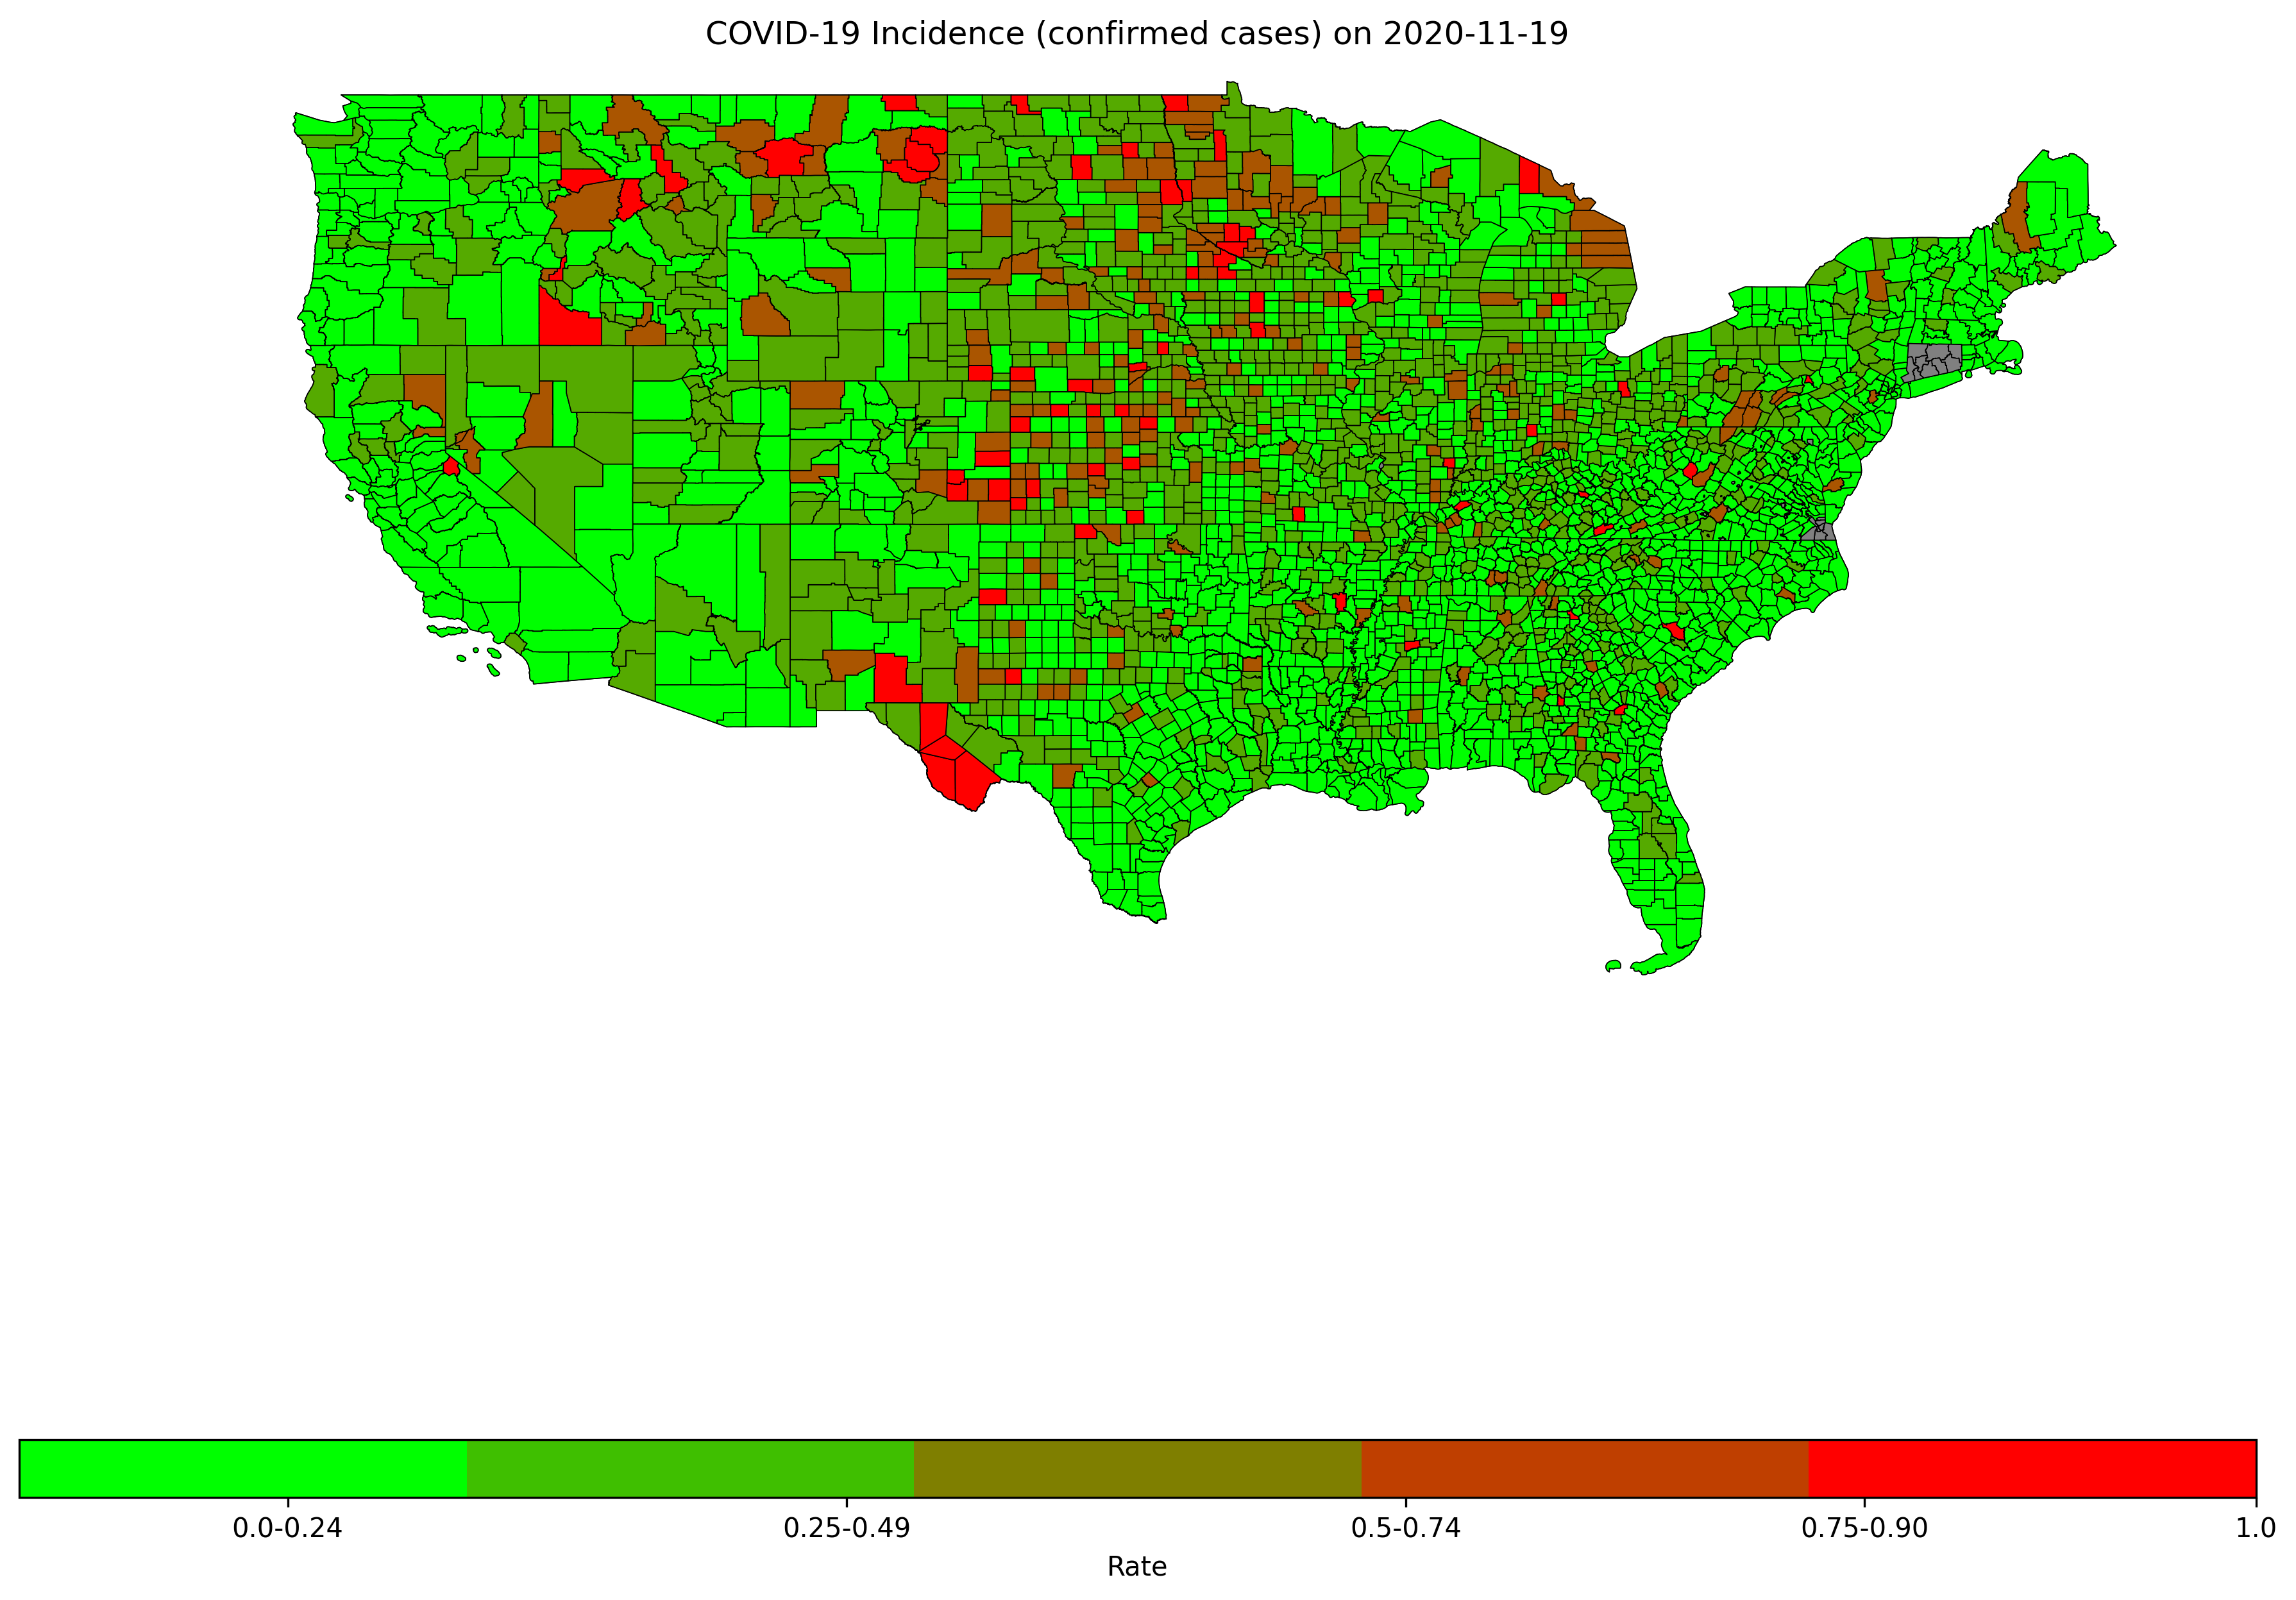
\includegraphics[width=1\linewidth]{Figures/IncidenceRate_covidCases2020-11-19.png}
  \caption{The displayed image reveals a notable spike in COVID-19 cases specifically in the mid-north region.}
  \Description{The aggregation was performed over 17 day intervals. }
\end{figure}

\begin{figure}[h]
  \centering
  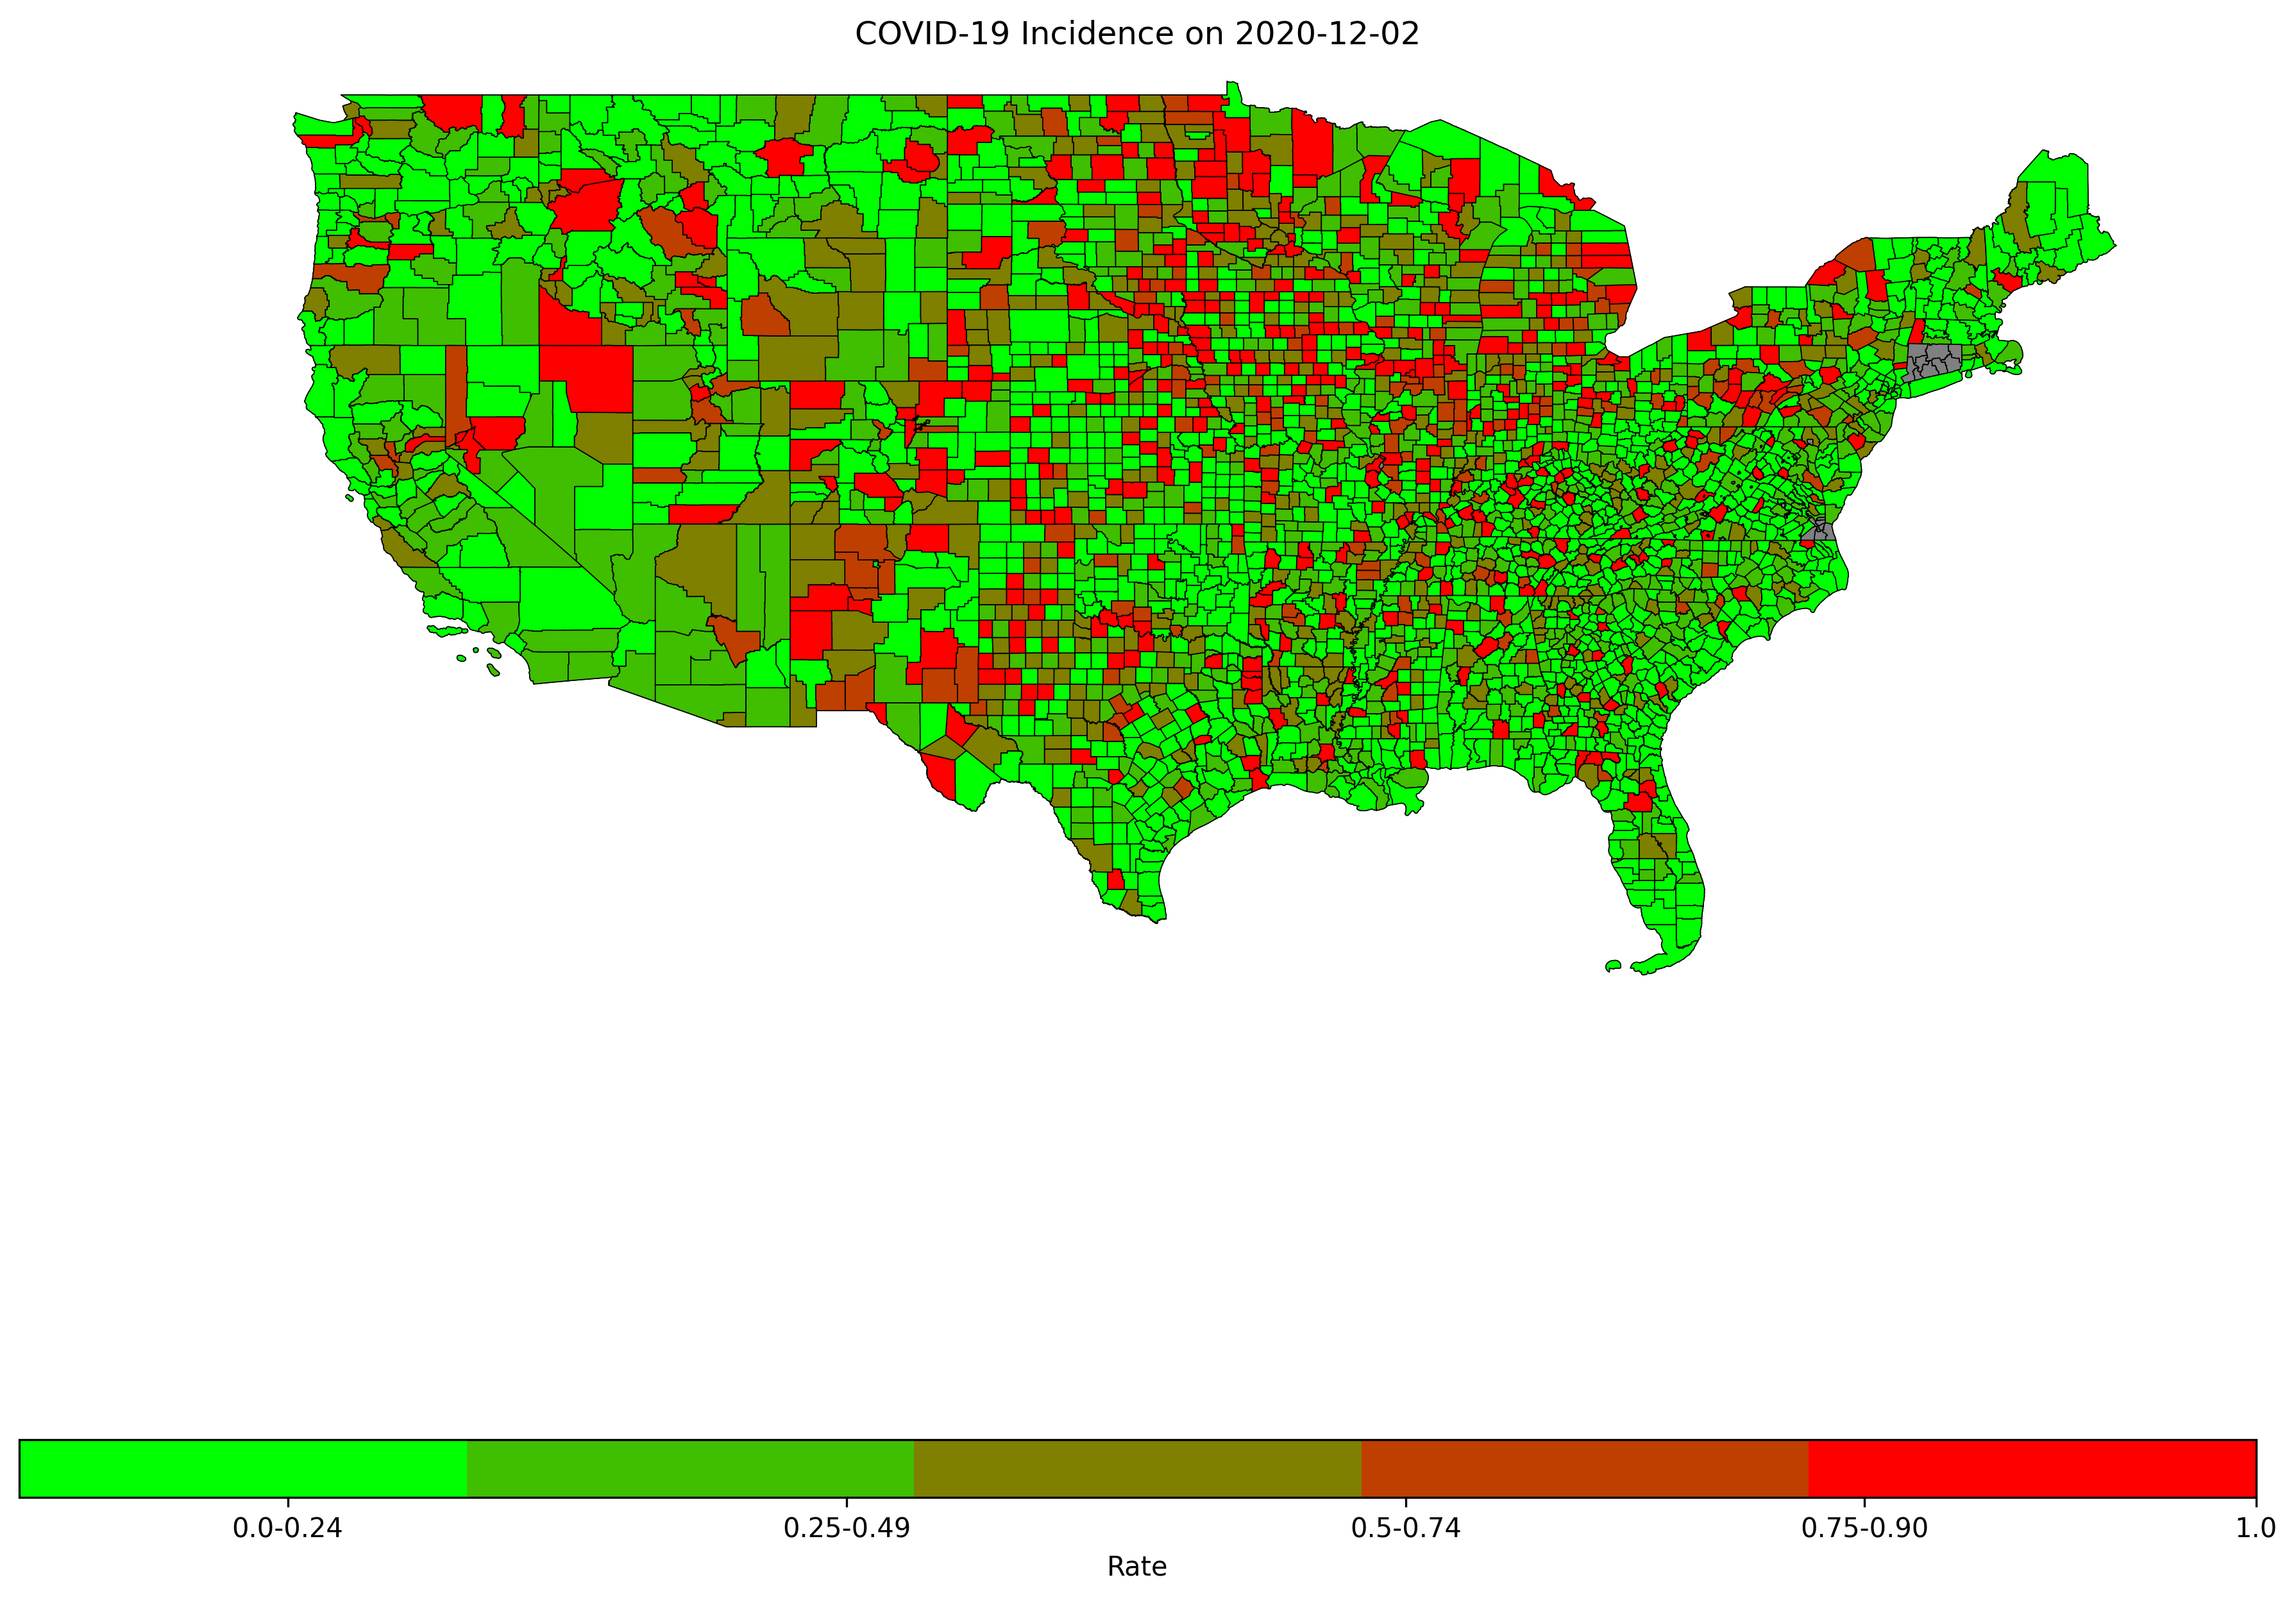
\includegraphics[width=1\linewidth]{Figures/IncidenceDeathRate_2020-12-02.png}
  \caption{The above image shows a spike in deaths for the mid-north region.}
  \Description{The aggregation was performed over 17 day intervals. }
\end{figure}



\begin{figure}[H]
  \centering
  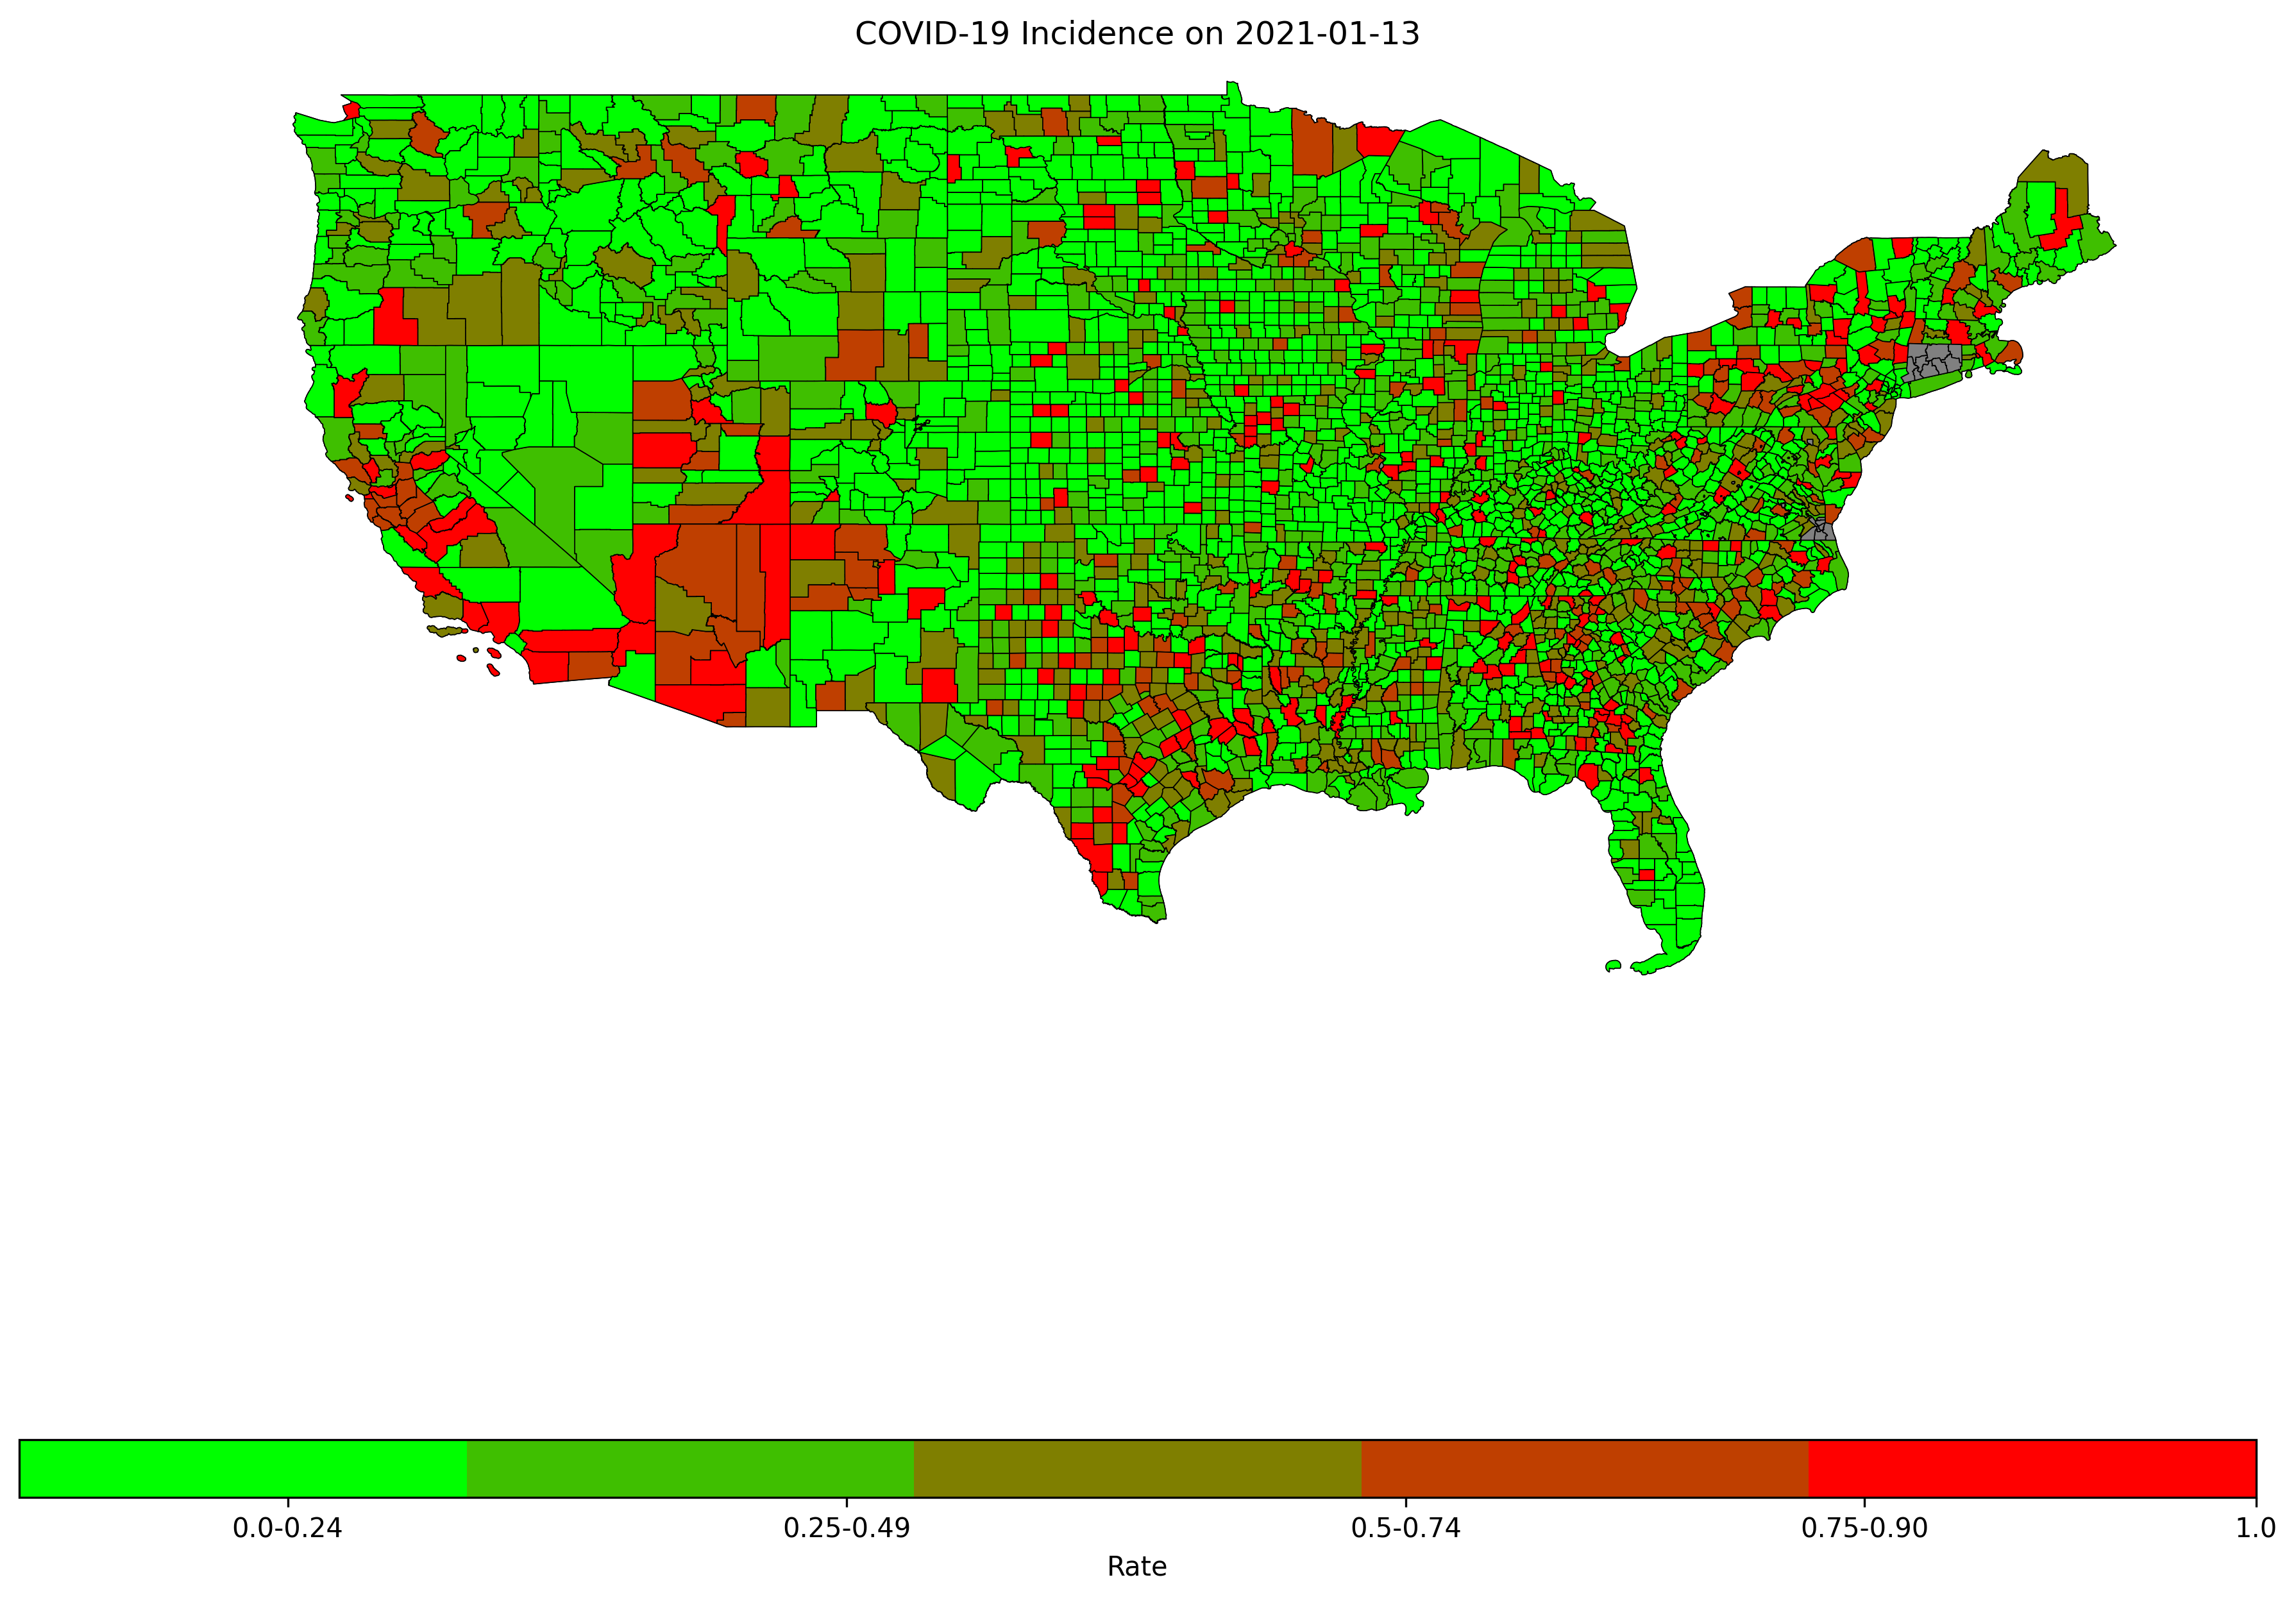
\includegraphics[width=1\linewidth]{Figures/IncidenceDeathRate_2021-01-13.png}
  
  \caption{We can see can see the results of an outbreak in the southwest region.}
  \Description{The aggregation was performed over 17 day intervals.}
\end{figure}
\noindent
The images in figure 1 and figure 2 display the death rate and confirmed cases across different counties, aggregated over 17-day intervals. We considered population size in our calculations, but it's also important to note that some states assign larger land areas to counties.

\begin{figure}[h]
  \centering
  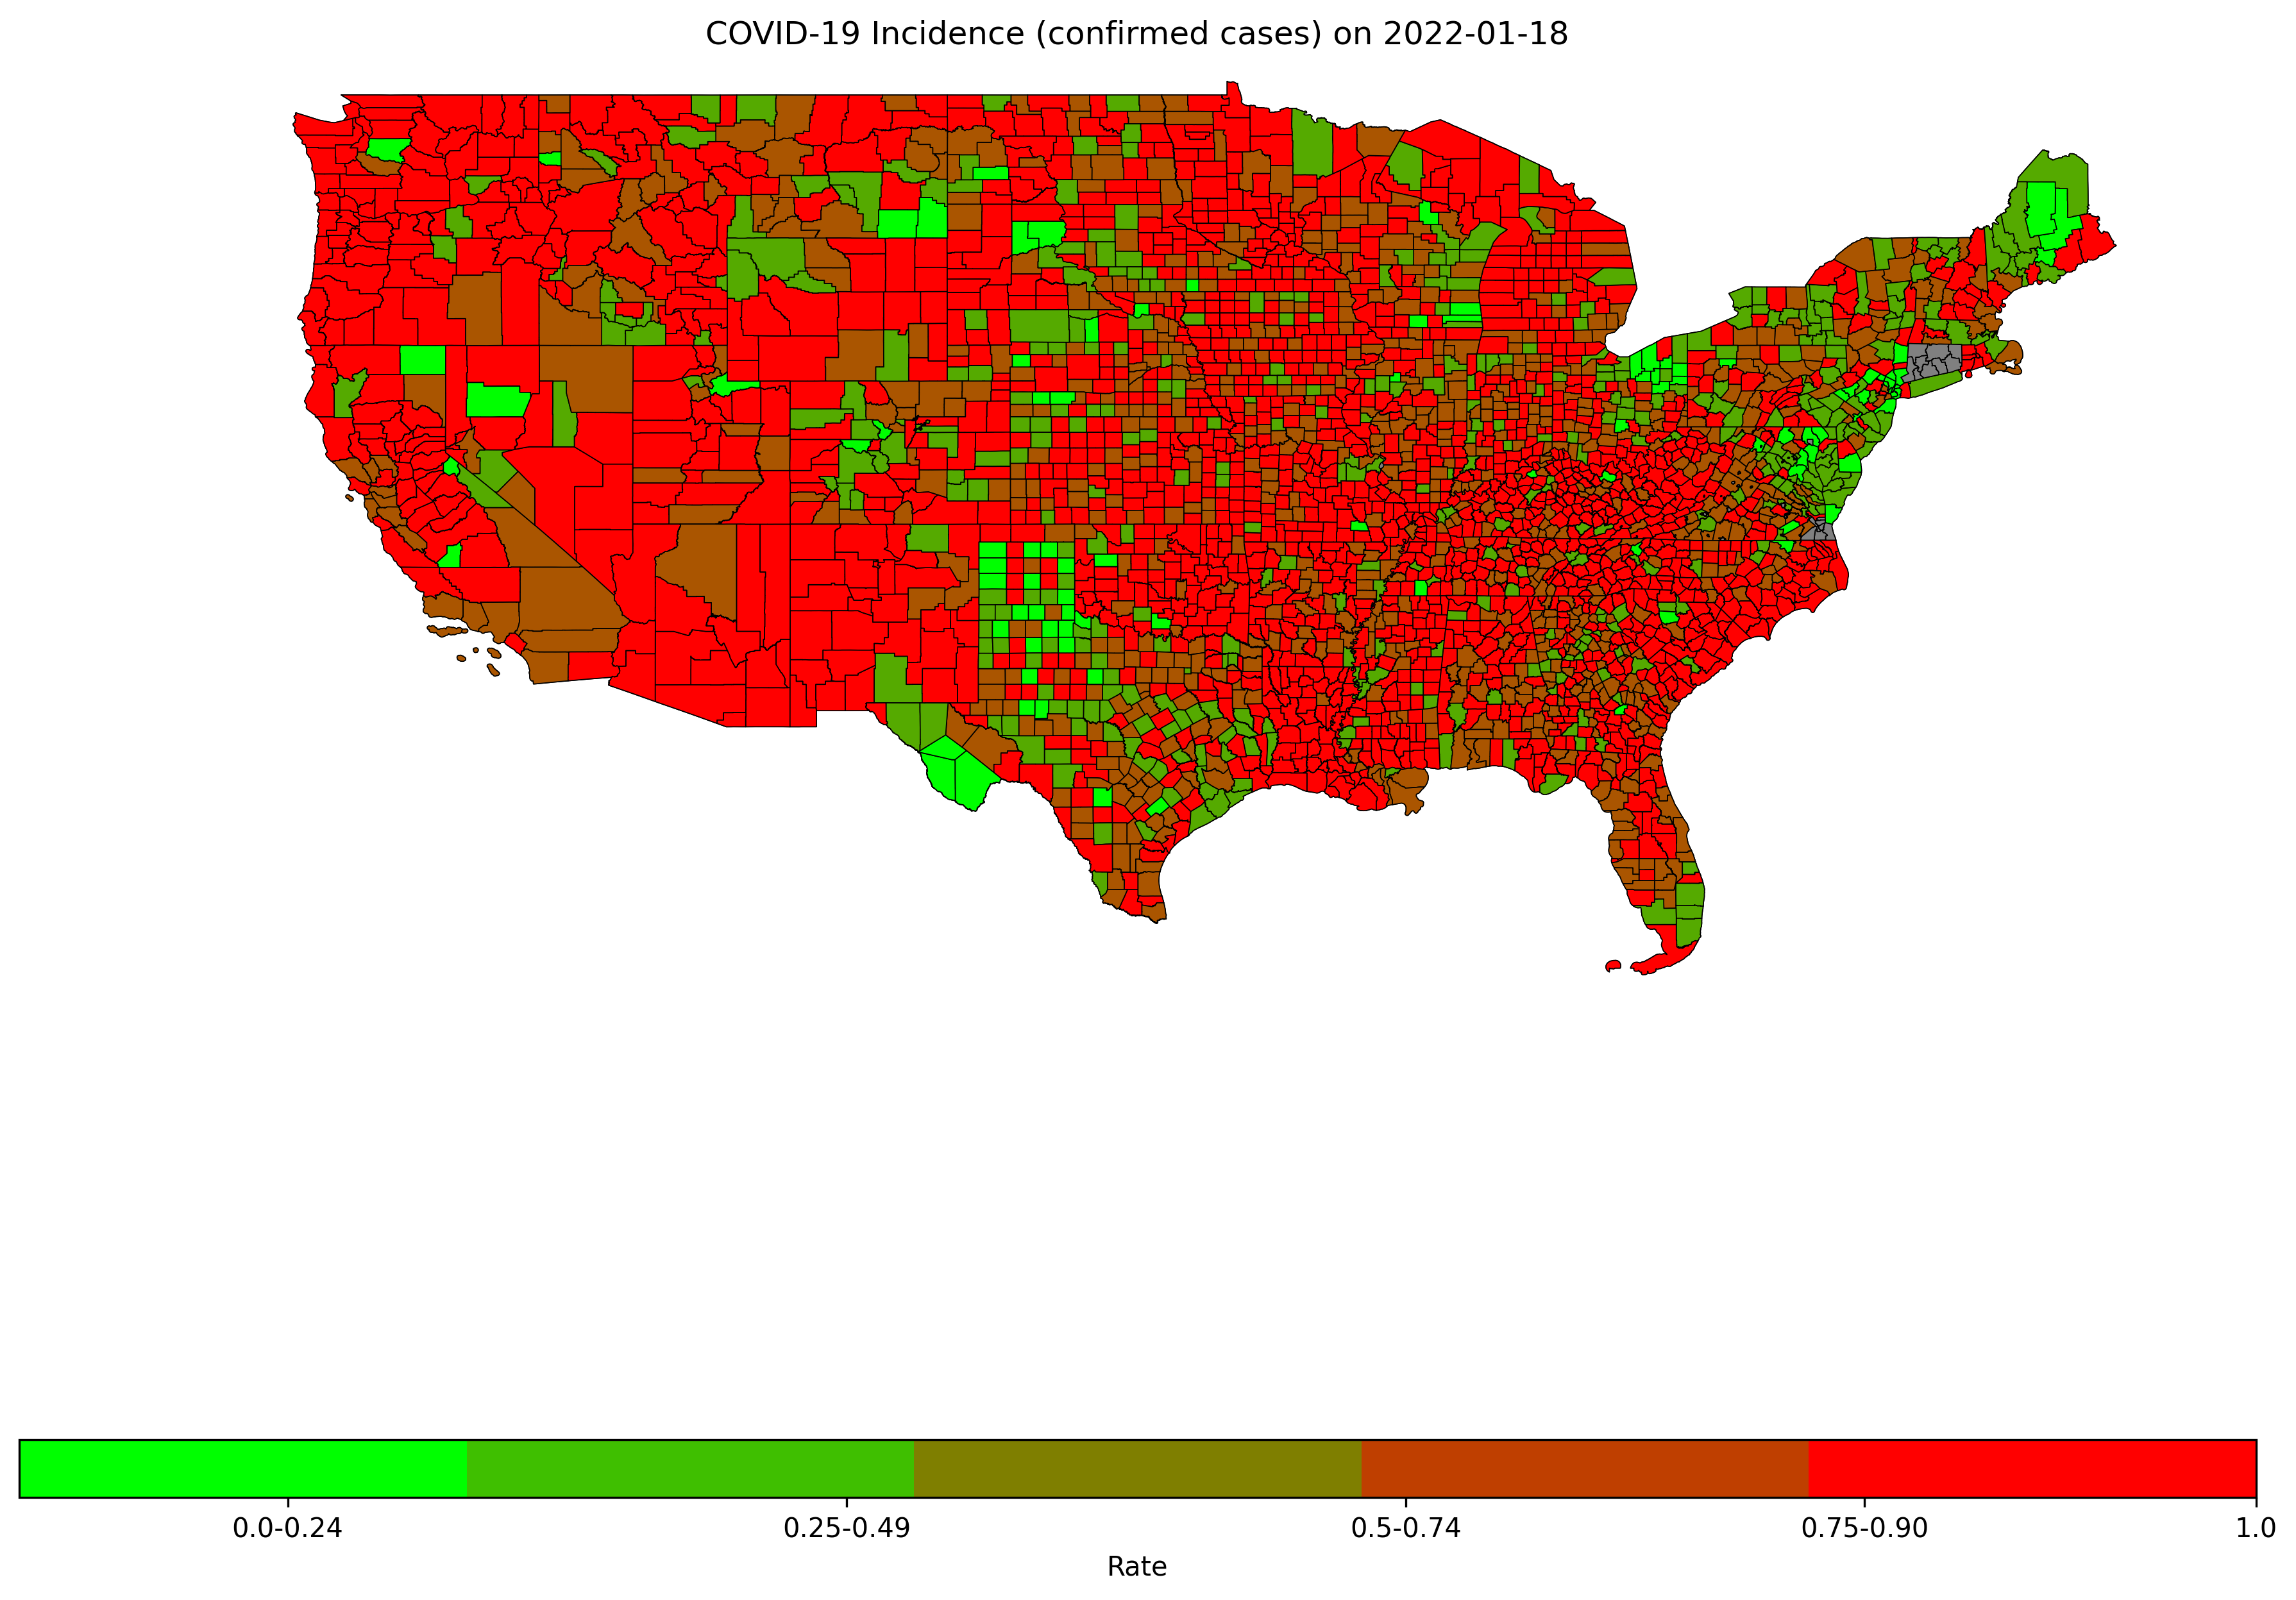
\includegraphics[width=1\linewidth]{Figures/IncidenceRate_covidCase_2022-01-18.png}
  
  \caption{COVID cases are seen here throughout the country.}
  \Description{There was a COVID outbreak across the country and we were trying to see comparison for death rate}
\end{figure}

\begin{figure}[H]
  \centering
  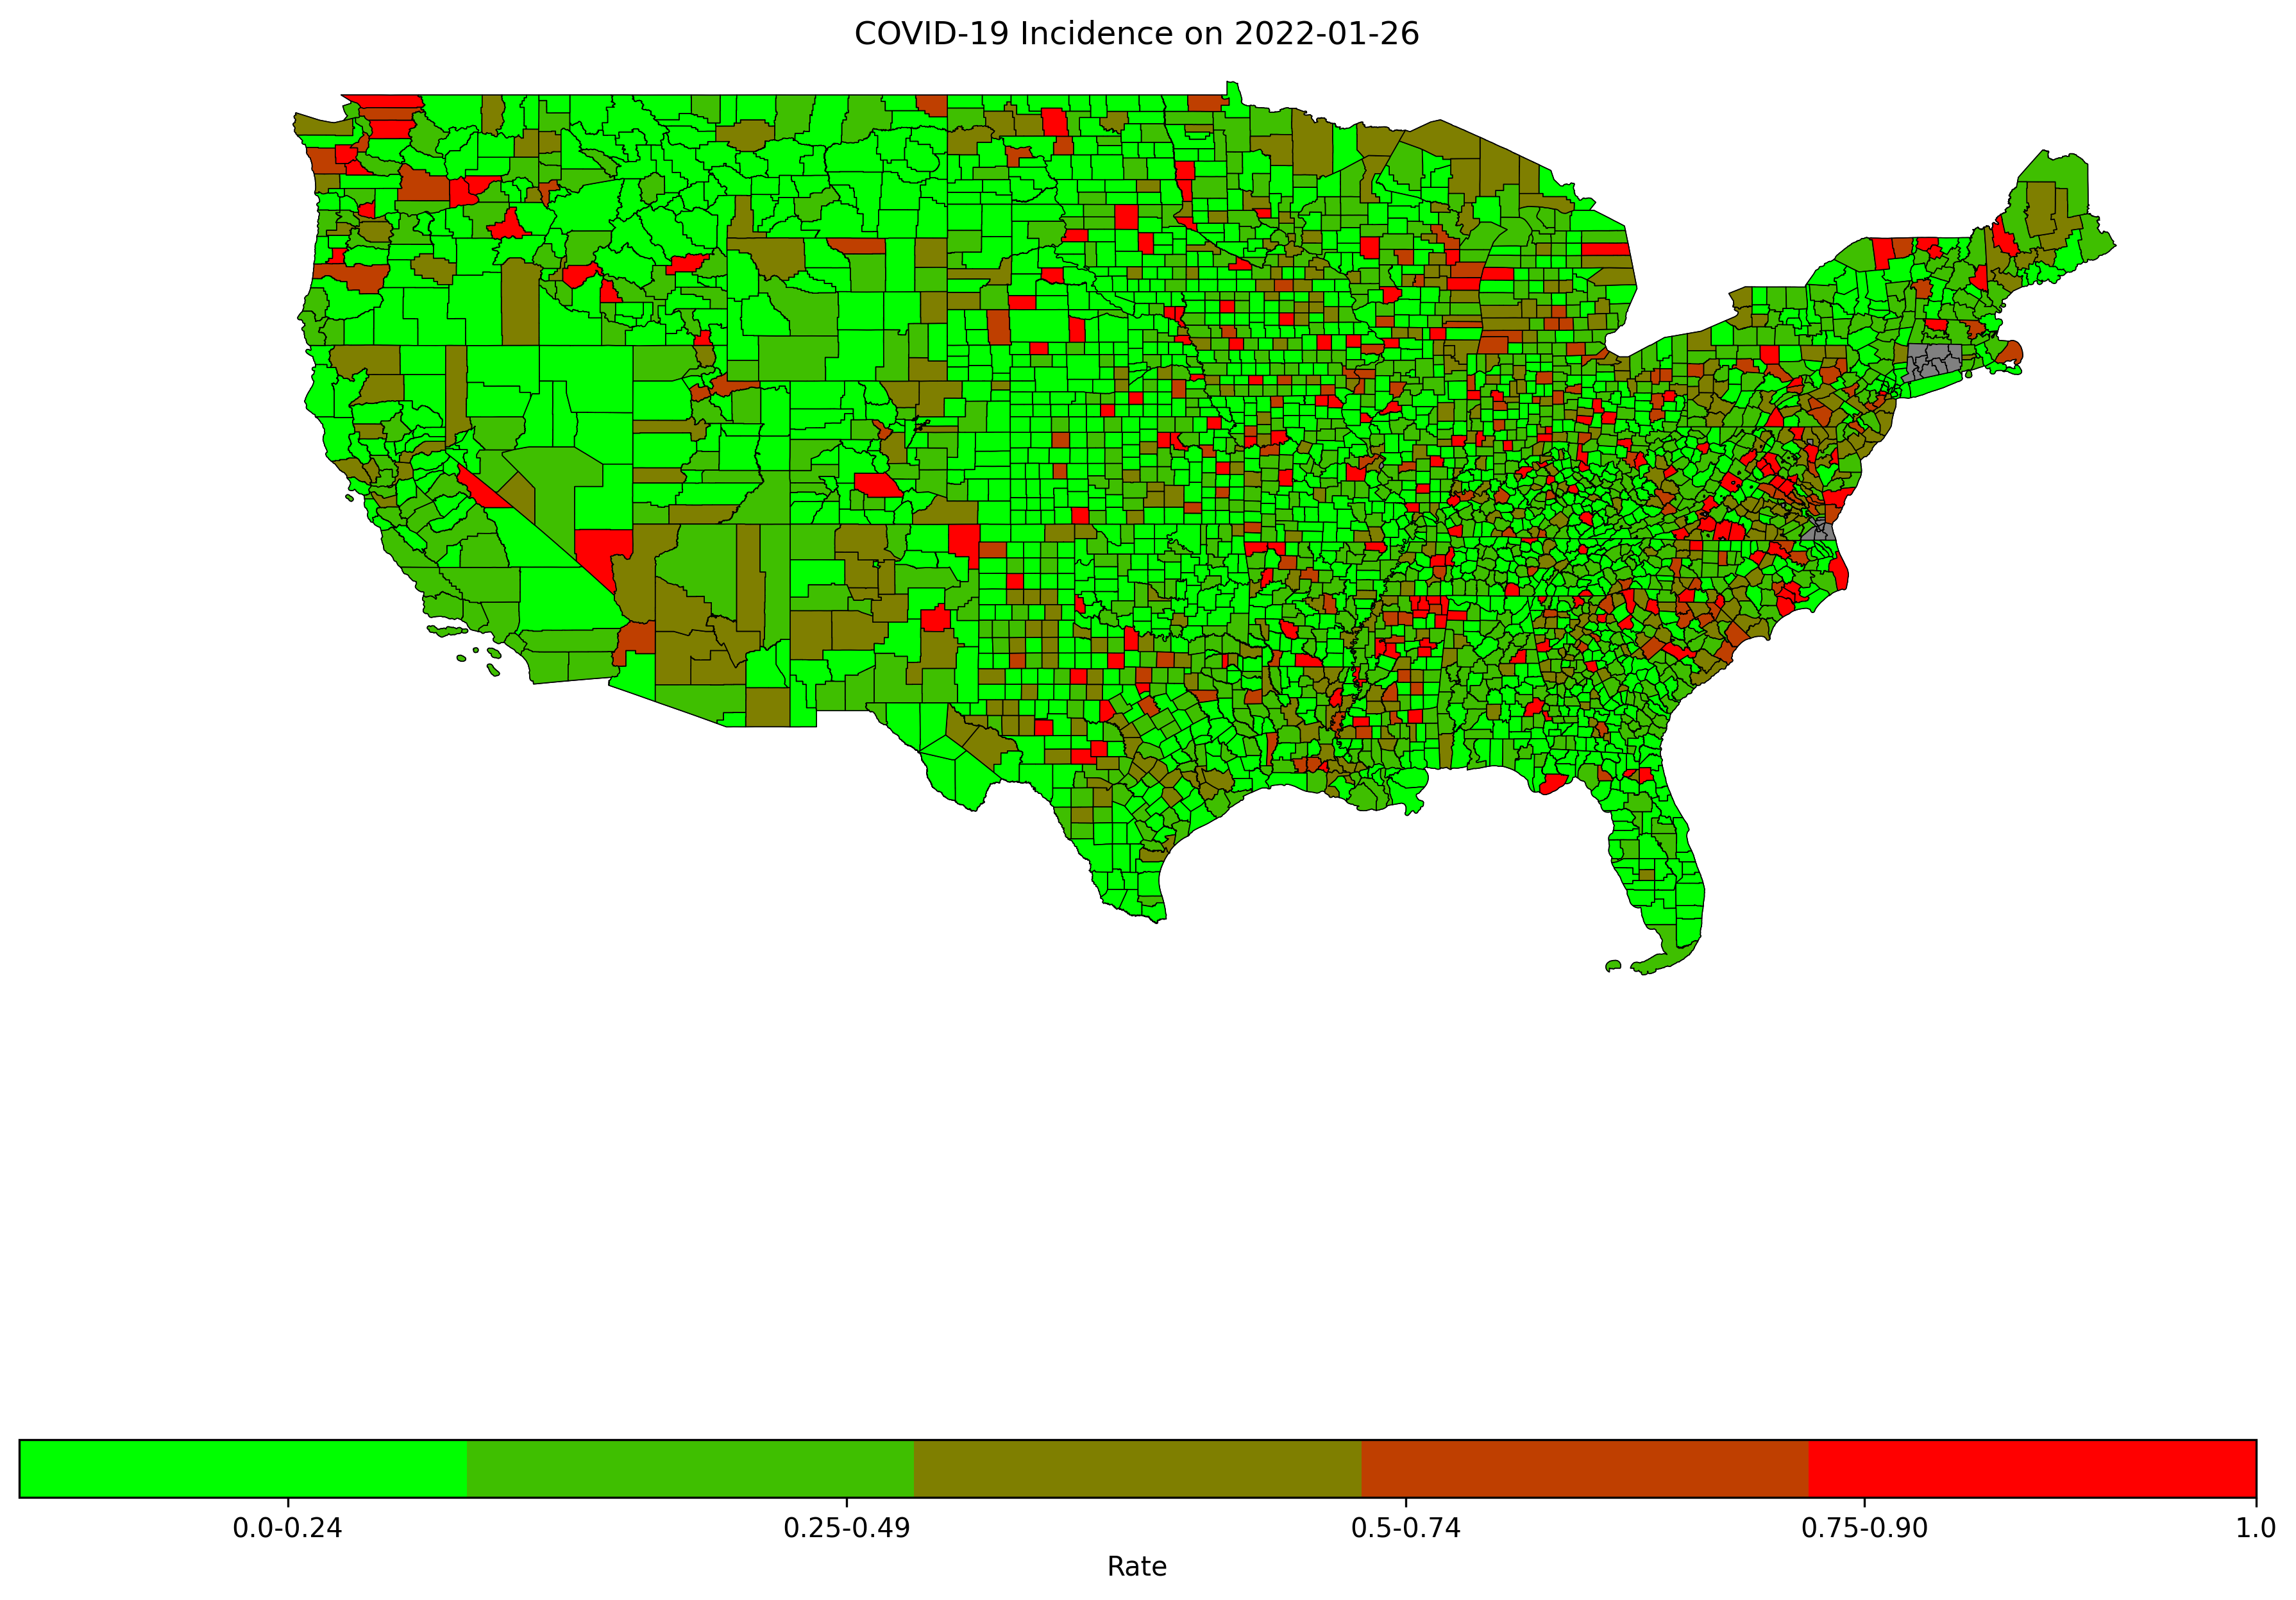
\includegraphics[width=1\linewidth]{Figures/IncidenceDeathRate_2022-01-26.png}
  \caption{Incident rate with relation to deaths.}
  \Description{There was a COVID outbreak across the country and we were trying to see comparison for death rate}
\end{figure}
\noindent
In Figure 4, there is a noticeable increase in the incidence of COVID-19 cases. However, Figure 5 indicates that although there is also a rise in deaths, it does not correspond proportionally to the spike in confirmed cases. This discrepancy suggests that vaccinations may have played a role in mitigating the severity of the virus.
\begin{figure}[H]
  \centering
  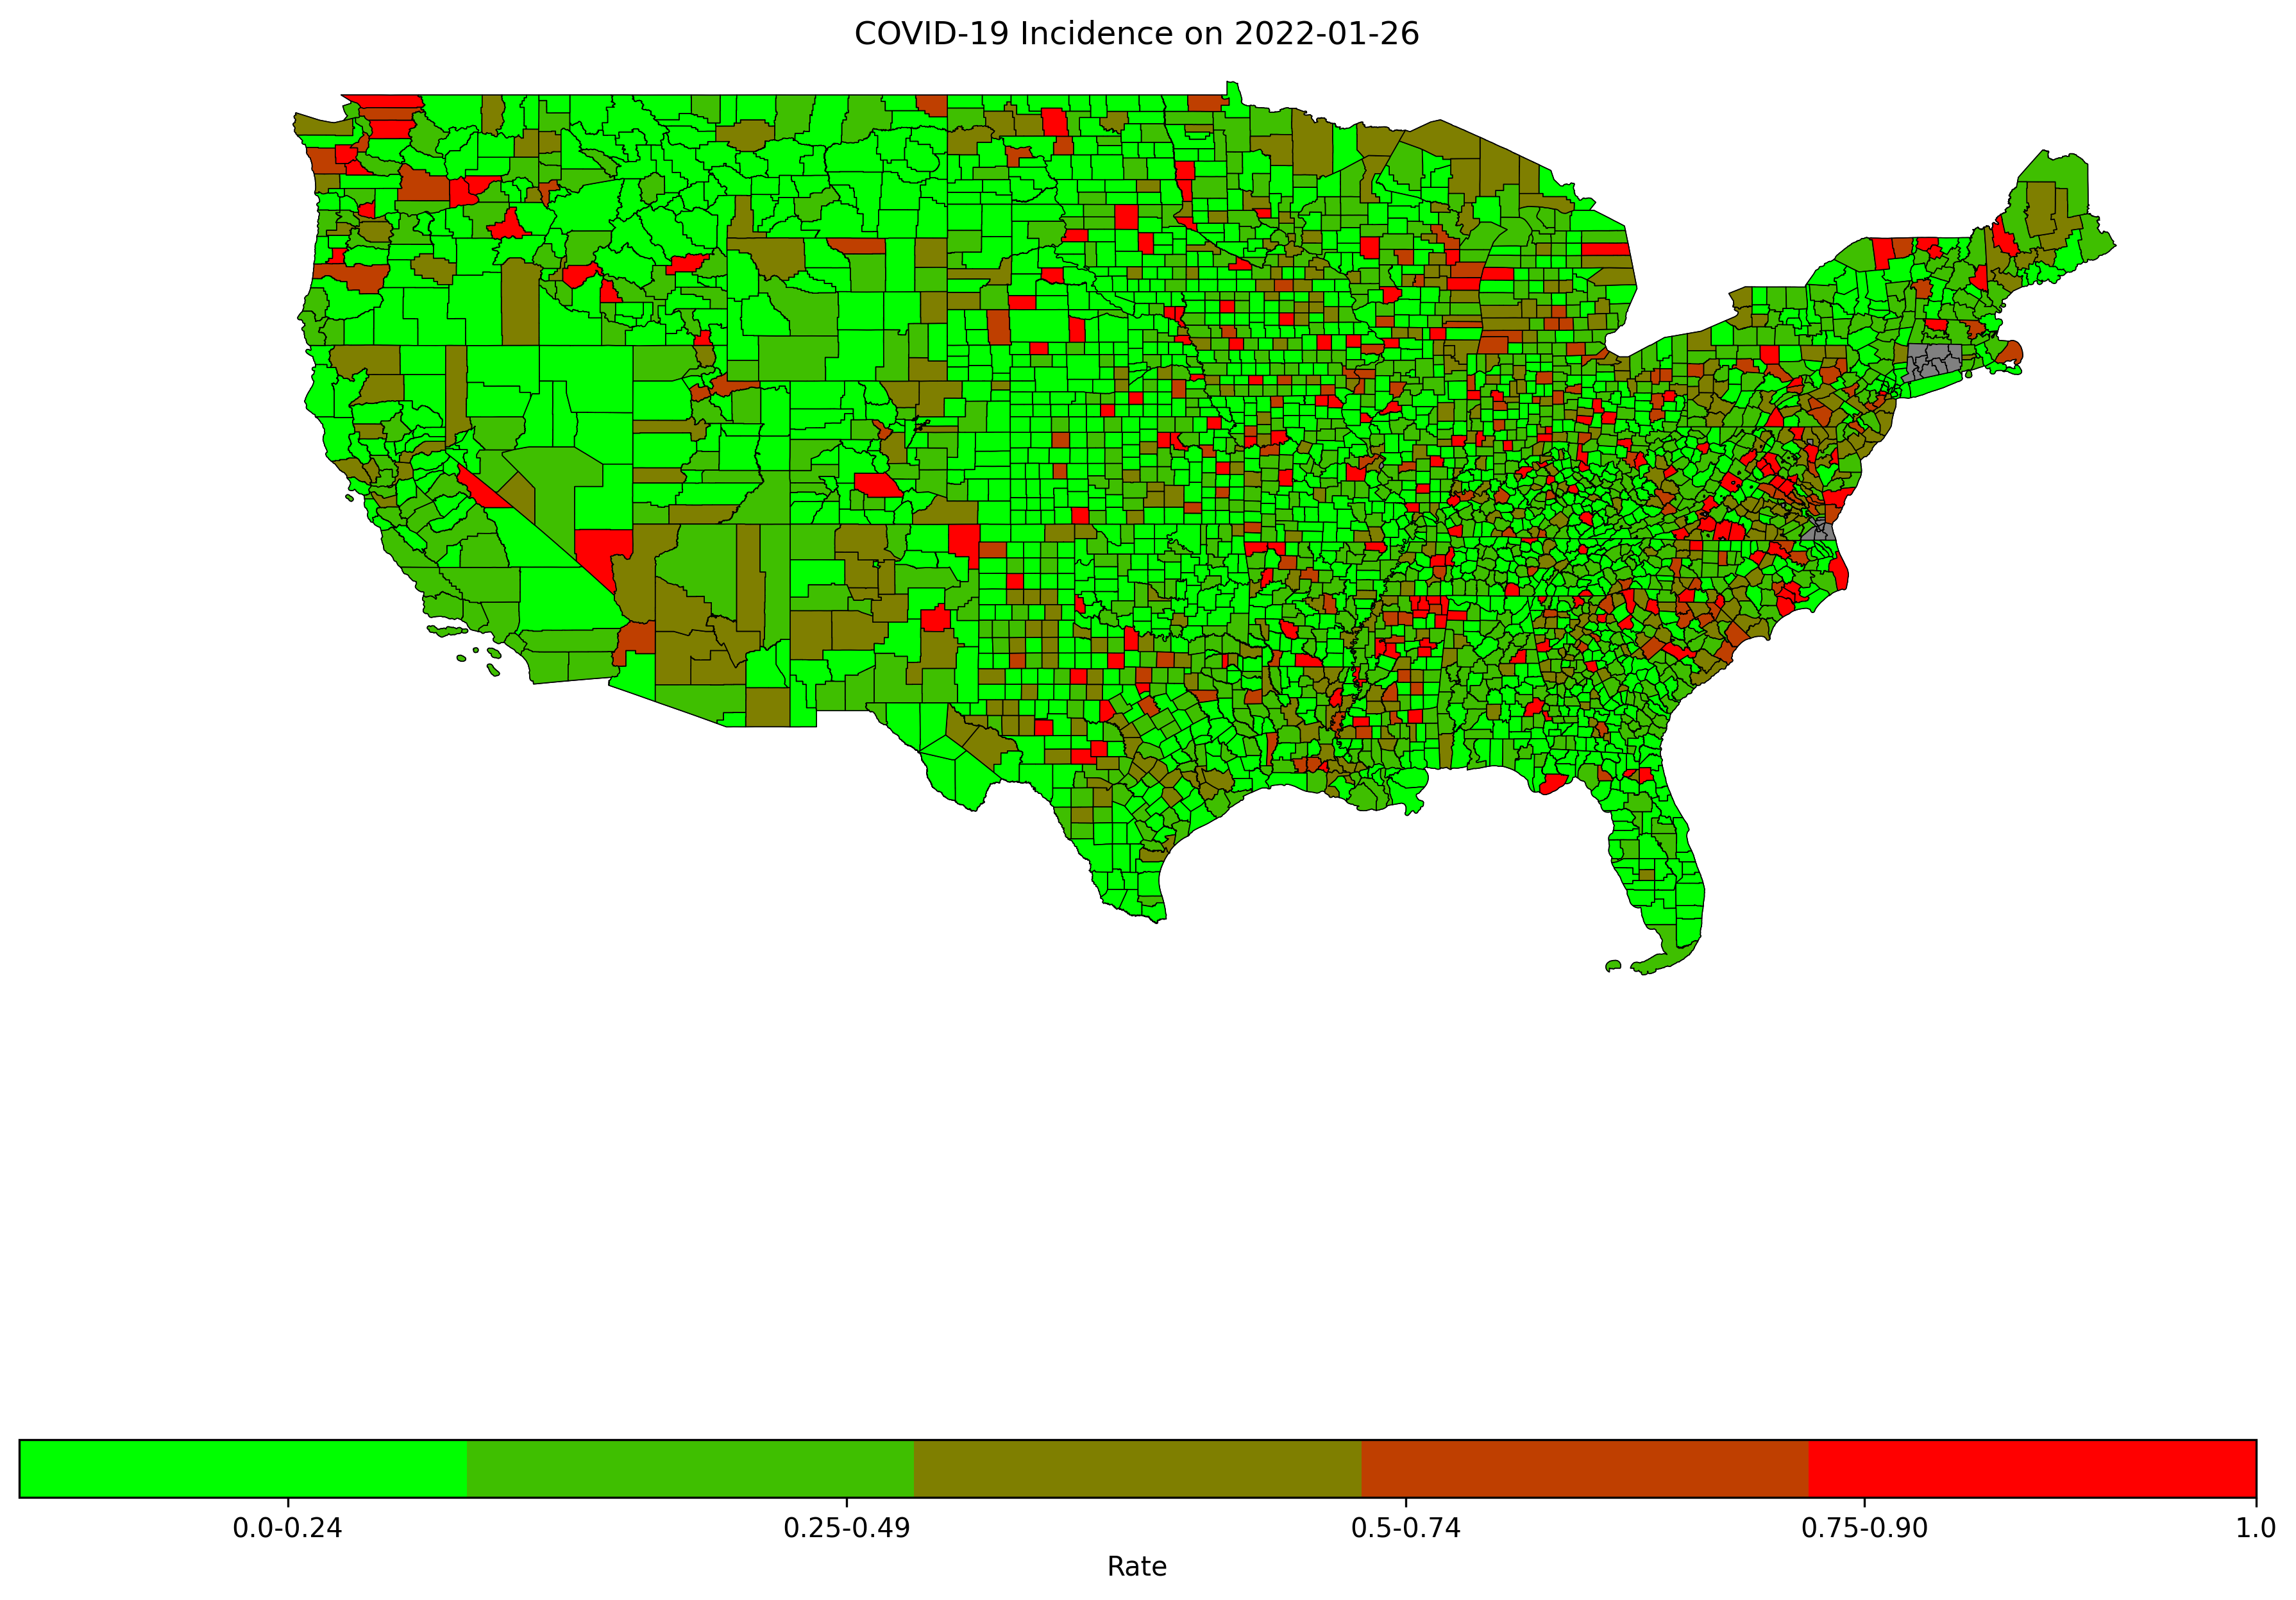
\includegraphics[width=1\linewidth]{Figures/IncidenceDeathRate_2022-01-26.png}
  \caption{Incident rate with relation to deaths.}
  \Description{There was a COVID outbreak across the country and we were trying to see comparison for death rate}
\end{figure}

\noindent
\subsection{Geospatial Analysis - Worst Counties During Worst Outbreaks}
Expanding on our Geospatial analysis, we looked at the worst counties during the worst outbreak periods on different aggregation periods. On the one-month aggregation level, December 2020 through February 2021 was the worst three-month period of the dataset. December 2020 had a nationwide COVID death toll of 77,298, January 2021 had deaths totaling 94,348, and February 2021 had deaths totaling 70,904. Of those months, Los Angeles County in California got hit the hardest, with 6,425 deaths in January 2021, and Maricopa County in Arizona coming in a distant second at 2,337 deaths that month. When the death tolls are separated into three bins, Los Angeles and Marcipa stand alone in their bins as the worst two death rates.

\begin{figure}[h]
  \centering
  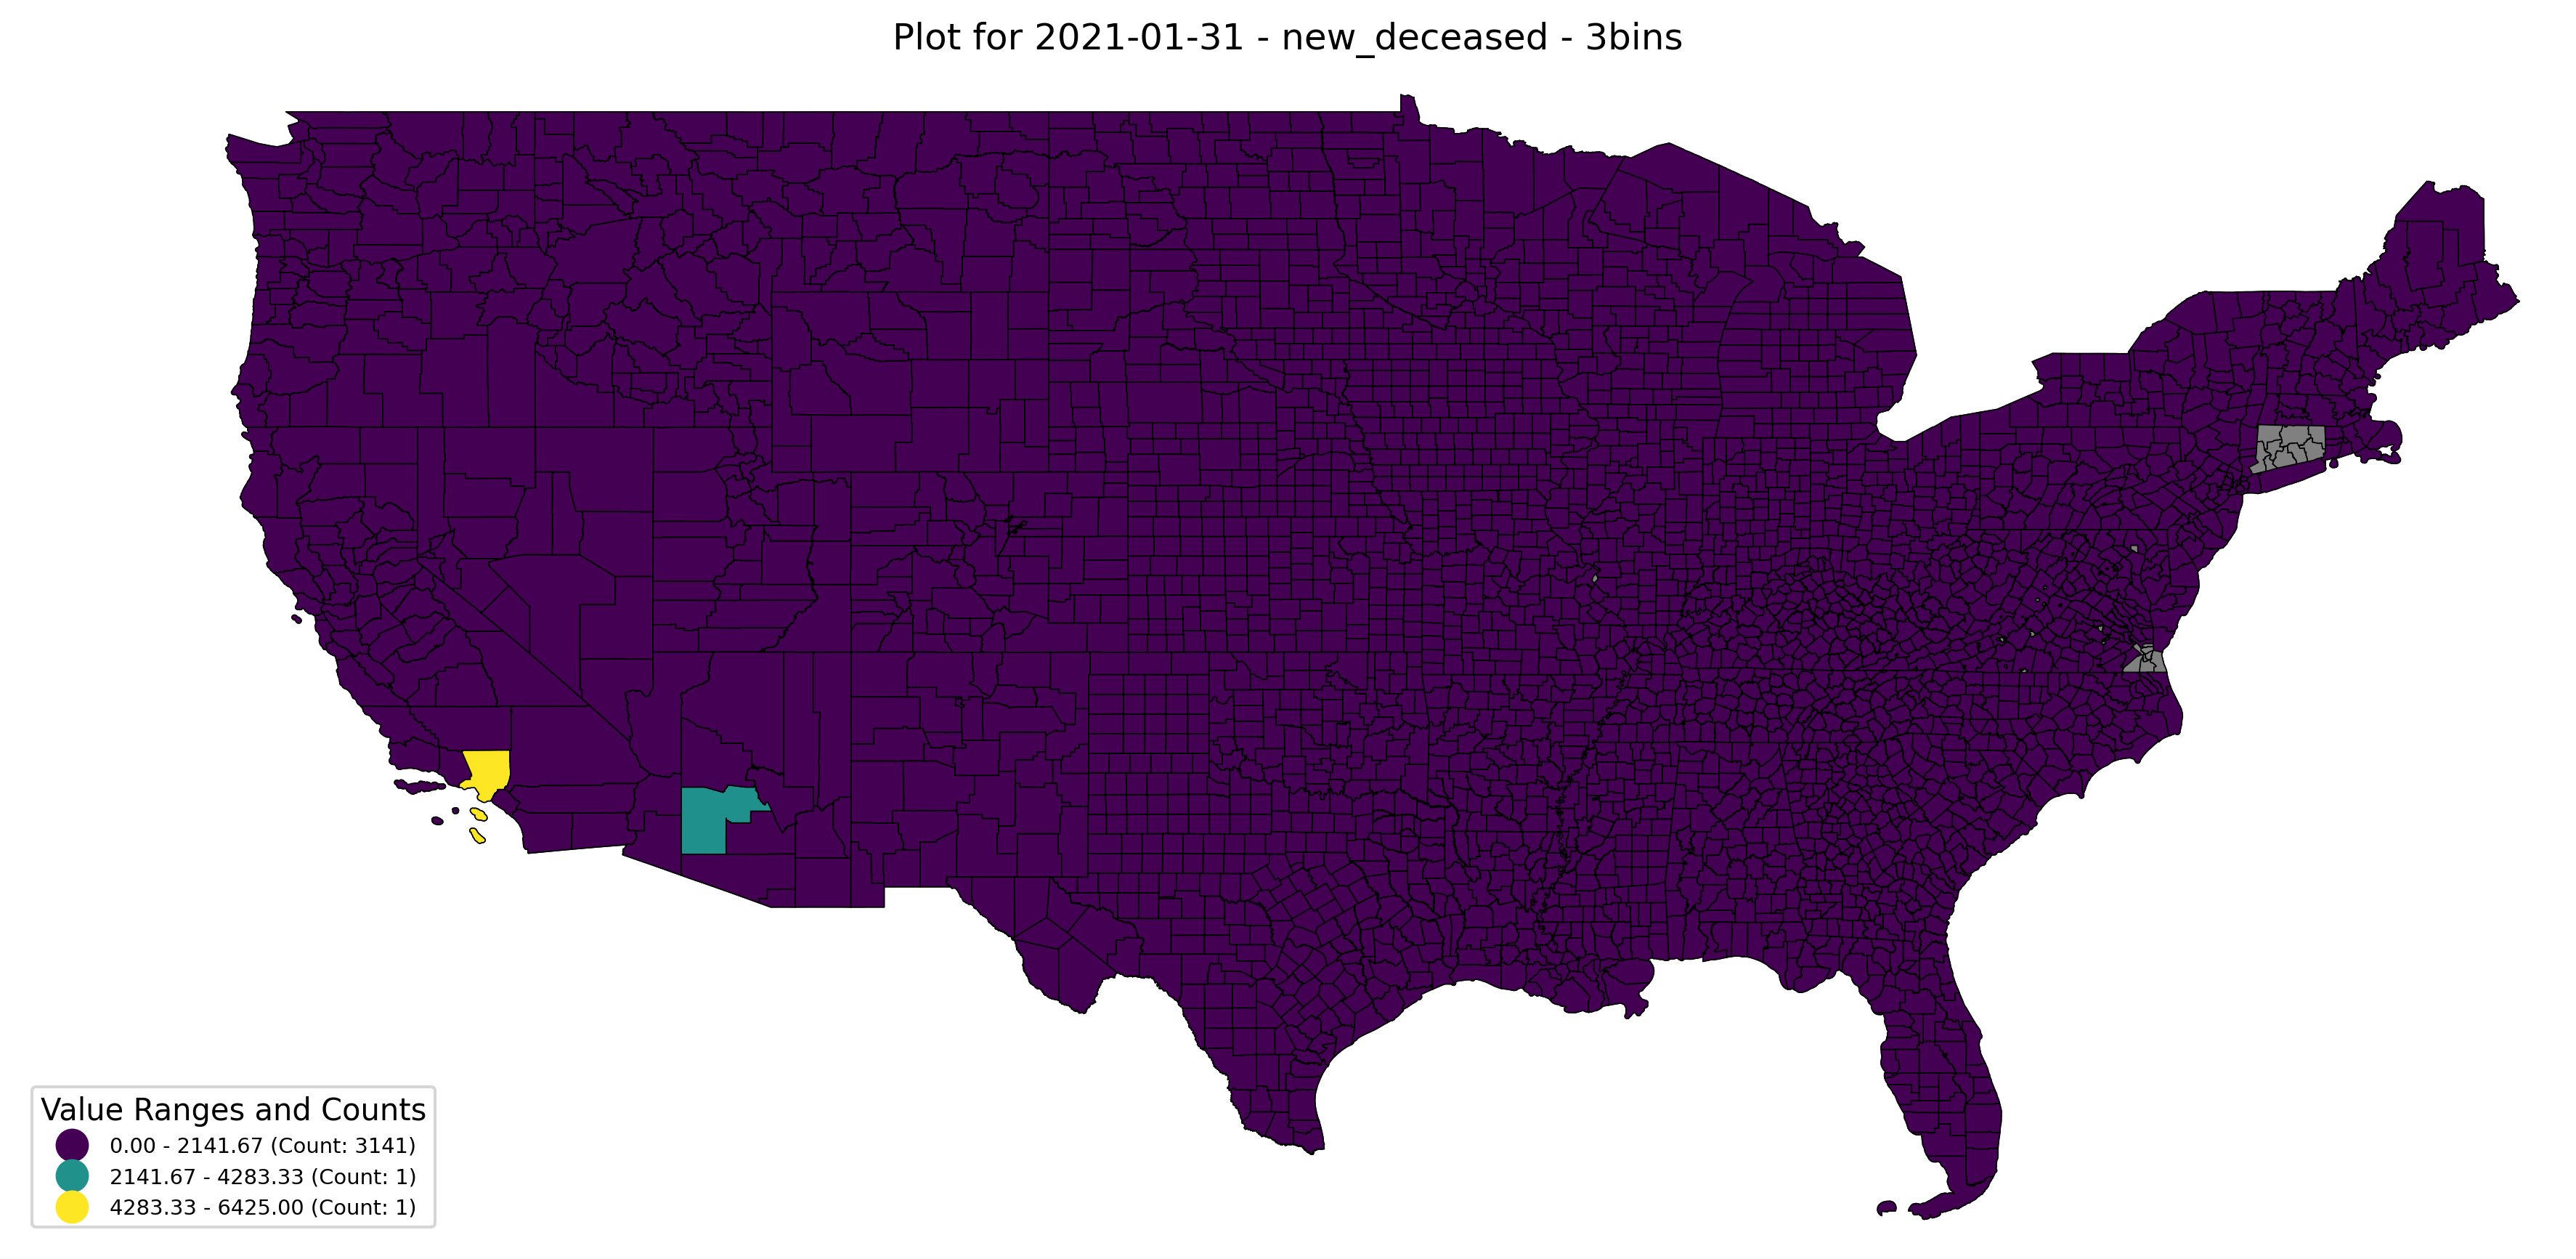
\includegraphics[width=1\linewidth]{Figures/Plot for Month Ending 2021-01-31 - new_deceased - 3bins.png}
  \caption{January 2021 Death Rate on One-Month Aggregation Level at Three Bins.}
  \Description{Los Angeles and Marcicopa County had the most deaths during one of the worst months of the dataset}
\end{figure}

When viewed as 10 bins, it shows that most of the worst counties after Los Angeles and Maricopa County were situated, for the most part, between and around those counties.

\begin{figure}[h]
  \centering
  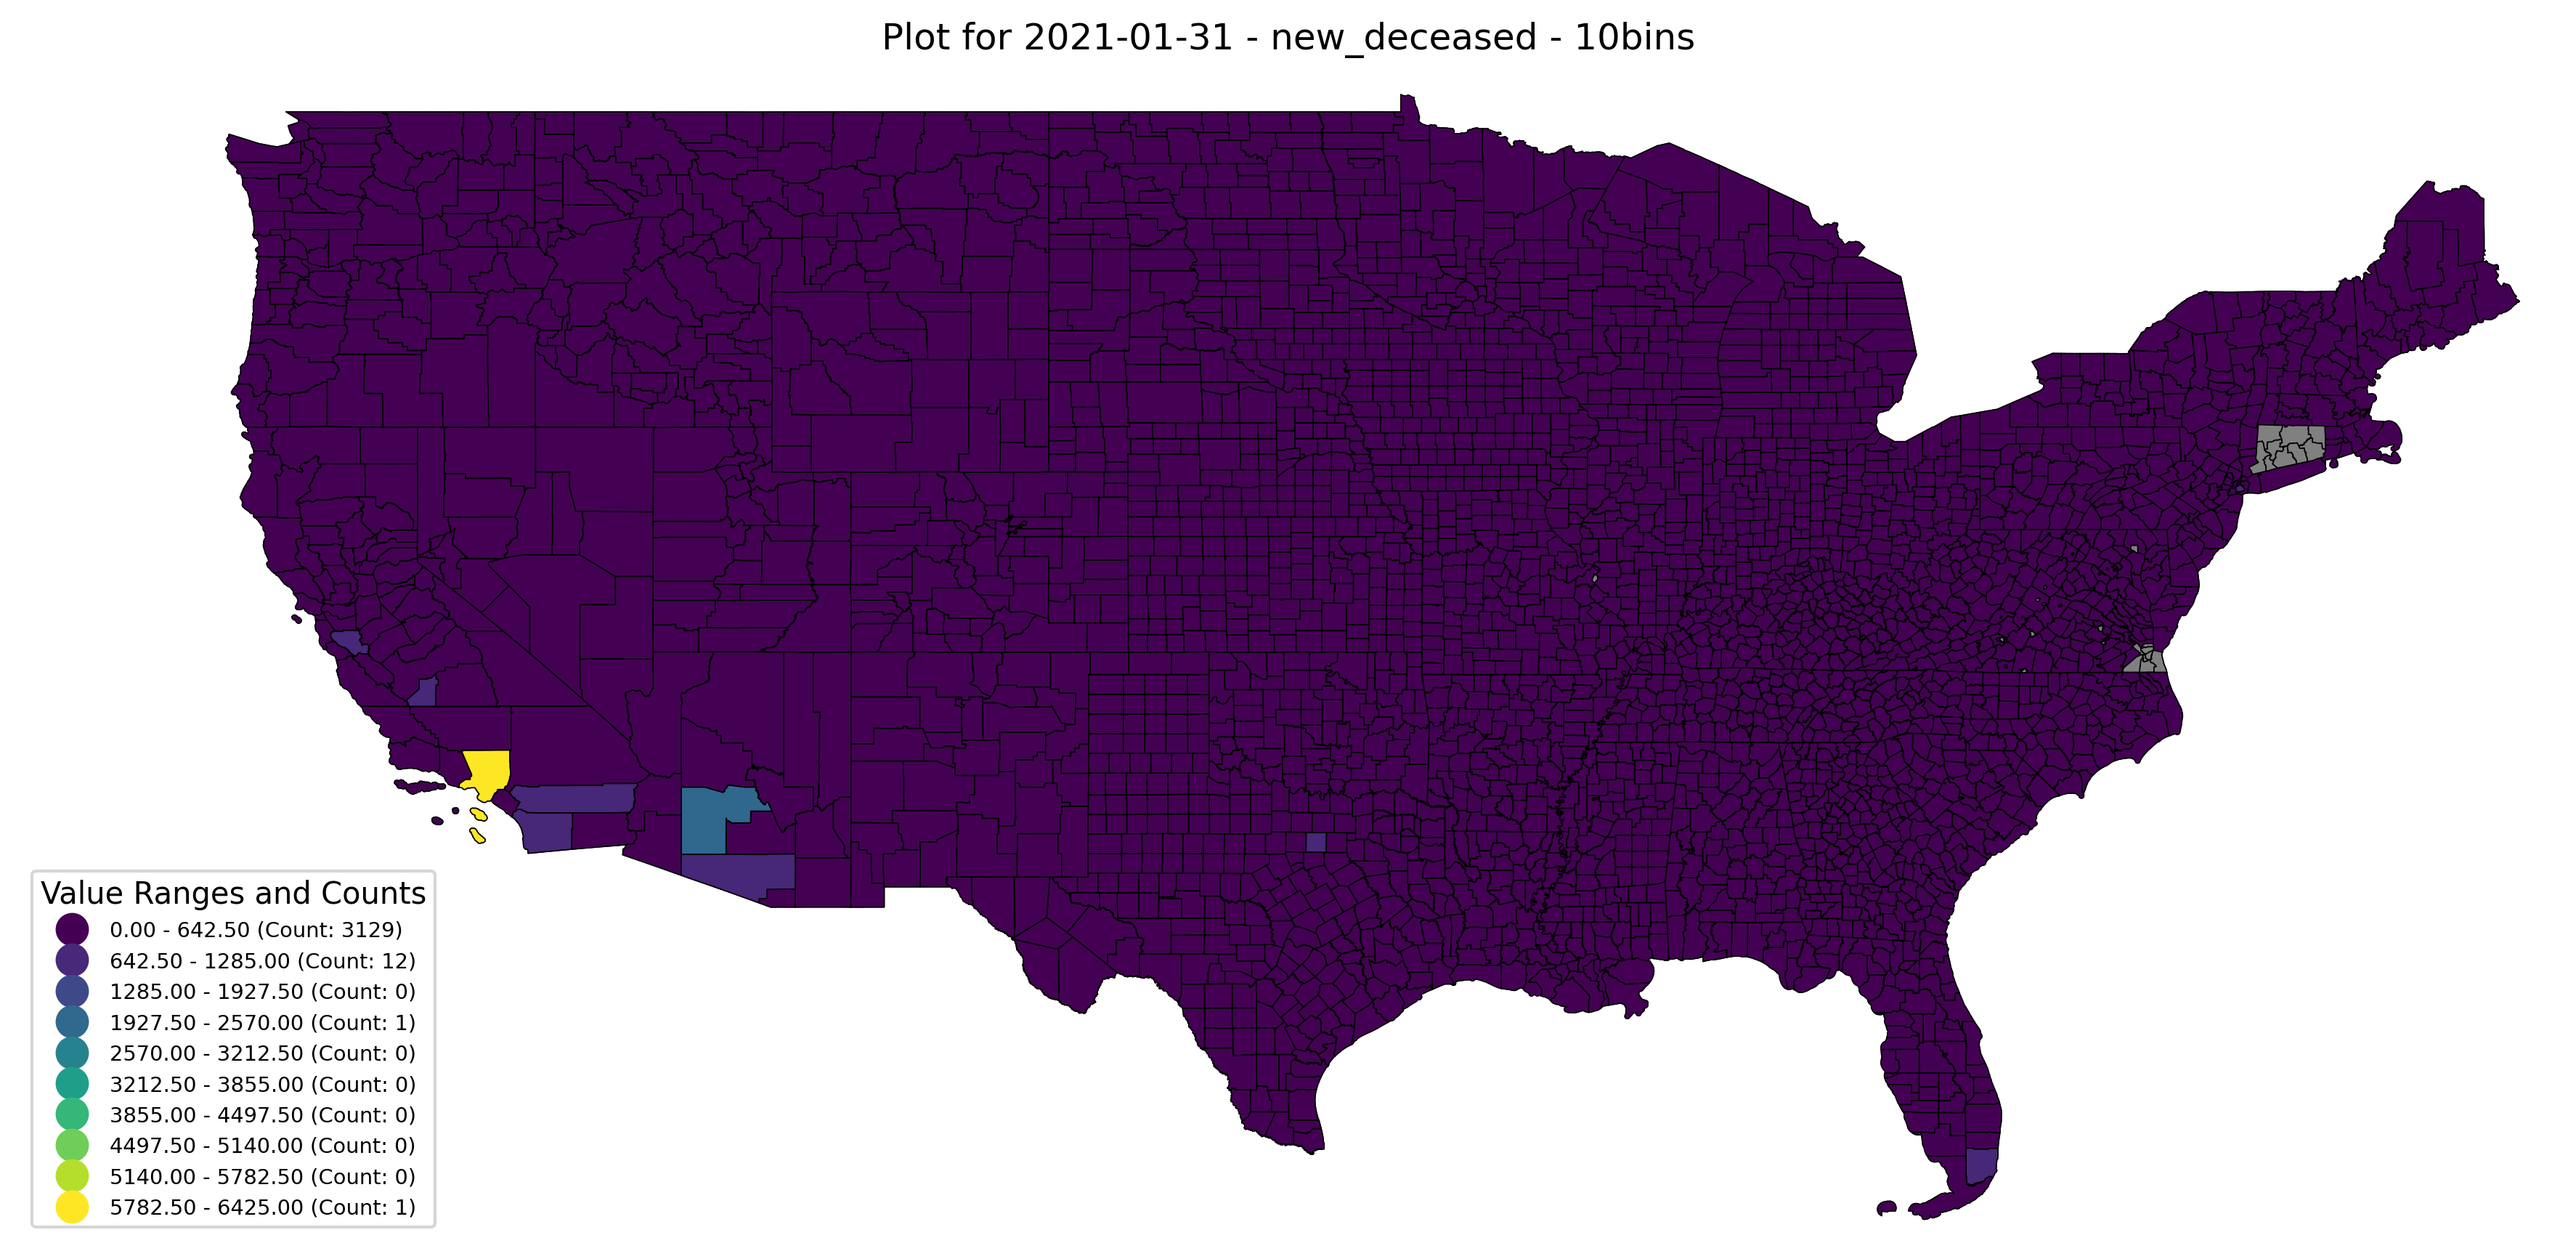
\includegraphics[width=1\linewidth]{Figures/Plot for Month Ending 2021-01-31 - new_deceased - 10bins.png}
  \caption{January 2021 Death Rate 10-bin Granularity Demonstrating Region Between Los Angeles and Maricopa had Worst Death Tolls after LA and Maricopa.}
  \Description{After Los Angeles and Marcicopa County, nearby areas were hit the worst}
\end{figure}

A similar situation can be found in Florida when viewed in shorter data timeframes. At a three-day interval, while most counties had less than 125 deaths per three-day period, the aggregation around September 13, 2021 shows that Florida experienced a significantly higher death tolls than the rest of the country, with one county exceeding 1,000 deaths over three days. When separated into 10 bins, the contrast is clear.

\begin{figure}[H]
  \centering
  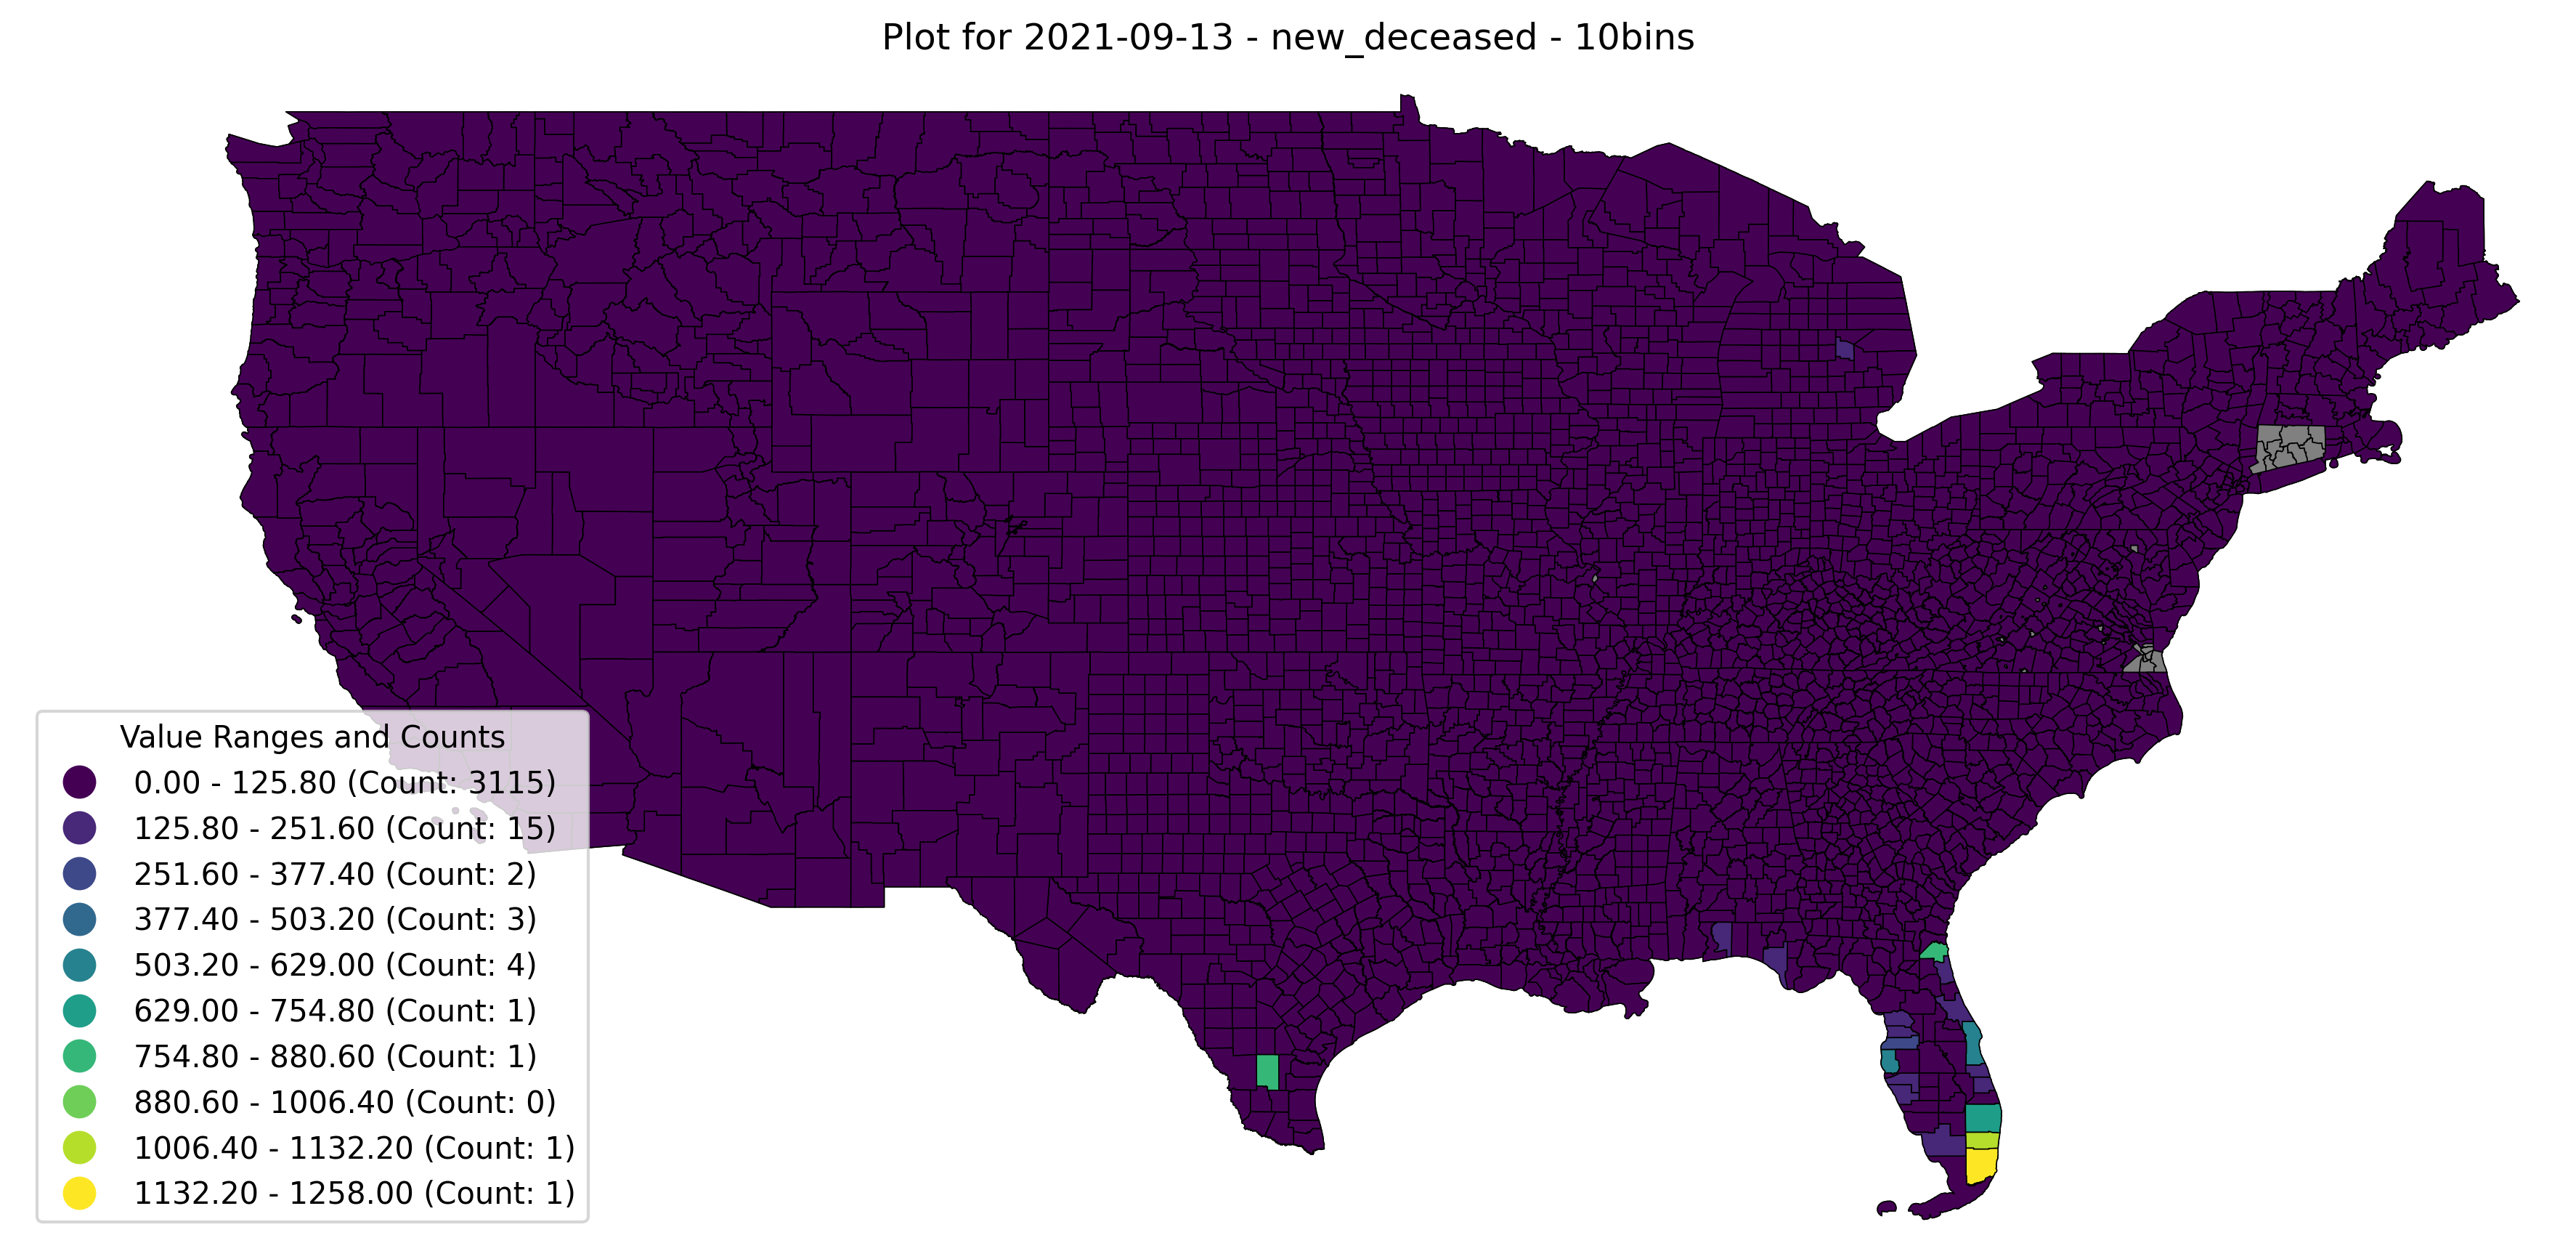
\includegraphics[width=1\linewidth]{Figures/Plot for 2021-09-13 - new_deceased - 10bins.png}
  \caption{September 2021 Death Rate 10-bin Granularity Shows Florida had Significantly Worse Death Tolls.}
  \Description{September 2021 Death Rate 10-bin Granularity Shows Florida had Significantly Worse Death Tolls.}
\end{figure}


% \newpage
\noindent
\subsection{Correlation analysis} \label{Sec:Corr}



The Pearson Correlation Coefficients for the variables shown in Table \ref{tab:correlation} were calculated to measure the linear relationship between confirmed COVID-19 cases and death rates with various environmental and mobility variables. These coefficients were computed using the built-in Pearson Correlation function of the \texttt{pandas} library in Python, which uses the following equation:

\begin{equation}
r = \frac{\sum (x_i - \overline{x})(y_i - \overline{y})}{\sqrt{\sum (x_i - \overline{x})^2 \sum (y_i - \overline{y})^2}}
\end{equation}

The coefficient quantifies the strength and direction of linear relation between two variables.

A correlation coefficient of -1, indicates a perfect negative linear correlation, while 0 for no correlation, and +1 for perfect positive correlation. The results are presented in Table \ref{tab:correlation} and are discussed below:

\begin{itemize}
    \item There is a moderate positive correlation ($r=0.24$) between the new confirmed cases and new deceased cases. This is consistent with expected trends in infectious disease outbreaks, indicating that increases in infections are typically accompanied by increases in deaths.
    \item Mobility data show weak negative correlations with new confirmed cases, with the highest in transit stations ($r=-0.099$) and workplaces ($r=-0.063$). This suggests that rising case numbers slightly reduce mobility in public and workplaces.
    \item Residential mobility shows a weak positive correlation ($r=0.087$) with new confirmed cases, indicating a slight increase in residential activity, possibly due to more people staying home during periods of high transmission.
    \item Temperature variables such as average, minimum and maximum temperatures all show weak negative correlations with new confirmed cases ($r$ values of $-0.029$, $-0.025$, and $-0.034$ respectively). This indicates a small impact of decreasing temperatures on the spread of the virus.
\end{itemize}

Most relationships are relatively weak, indicating the complex nature of pandemic dynamics.




\begin{table}[H]
\centering
\caption{Correlation coefficients between COVID-19 case metrics and various mobility and environmental variables.}
\begin{tabular}{lcc}
\hline
\textbf{Variable} & \textbf{New Confirmed} & \textbf{New Deceased} \\ \hline
new\_confirmed & 1.000000 & 0.240407 \\
new\_deceased & 0.240407 & 1.000000 \\
mobility\_retail\_and\_recreation & -0.068893 & -0.082005 \\
mobility\_grocery\_and\_pharmacy & -0.055497 & -0.067243 \\
mobility\_parks & -0.070682 & -0.062156 \\
mobility\_transit\_stations & -0.099402 & -0.102103 \\
mobility\_workplaces & -0.063318 & -0.066253 \\
mobility\_residential & 0.087180 & 0.099044 \\
average\_temperature\_celsius & -0.029875 & -0.014980 \\
minimum\_temperature\_celsius & -0.025170 & -0.009587 \\
maximum\_temperature\_celsius & -0.034440 & -0.021168 \\
rainfall\_mm & -0.005717 & -0.003457 \\
dew\_point & -0.031608 & -0.019824 \\
relative\_humidity & -0.008104 & -0.011446 \\ \hline
\end{tabular}
\label{tab:correlation}
\end{table}




Figure \ref{fig:scatter-cor} shows the scatter plot of the new COVID-19 cases and the average temperature in Celsius across different counties. The distribution does not indicate a strong linear relationship, as the data points are spread across the whole temperature range without a clear pattern. 


\begin{figure}[H]
  \centering
  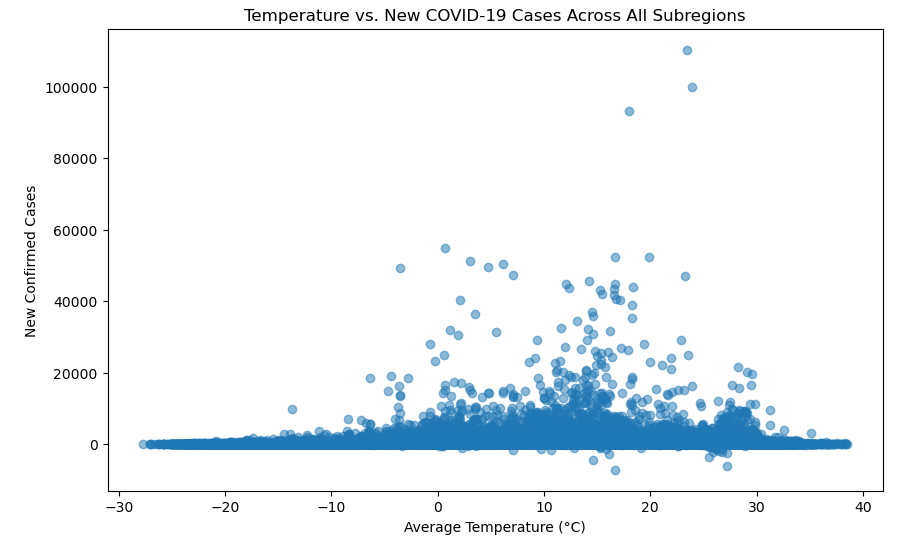
\includegraphics[width=\linewidth]{Figures/Correlation-scatter.PNG}
  \caption{Scatter plot of new COVID-19 cases against average temperature for all counties.}
  \Description{Scatter plot of new COVID-19 cases against average temperature for all counties}
  \label{fig:scatter-cor}
\end{figure}

% \newpage
\noindent
\subsection{Comparative Regression Analysis with and without Lagged Variables - Ordinary Least Squares} \label{Sec:ComparativeRegr}

This analysis explores the impact of incorporating lagged variables into our regression model to predict new COVID-19 cases based on environmental and mobility data. Initially, a basic model excluding lagged variables was utilized to set a baseline for performance comparison.

\subsubsection{Initial Model without Lagged Variables}
The initial regression model used the following predictors: average temperature, minimum temperature, maximum temperature, rainfall, and relative humidity. This model provided a baseline understanding of the relationship between these environmental factors and COVID-19 transmission.

\begin{equation}
Y = \beta_0 + \beta_1X_1 + \beta_2X_2 + ... + \beta_5X_5 + \epsilon
\end{equation}

where \( Y \) represents new confirmed cases per 1000 people, and \( X_1 \) to \( X_5 \) are the environmental predictors. The model results were as follows:

\begin{table}[H]
\centering
\caption{OLS Regression results without lagged predictors.}
\label{tab:regression_results_initial}
\begin{tabular}{lcccc}
\hline
\textbf{Variable} & \textbf{Coefficient} & \textbf{Std. Error} & \textbf{t-value} & \textbf{P>|t|} \\
\hline
Constant & 2.2900 & 0.064 & 35.845 & 0.000 \\
Average Temp. (°C) & -0.8450 & 0.012 & -71.910 & 0.000 \\
Min Temp. (°C) & 0.3907 & 0.007 & 55.921 & 0.000 \\
Max Temp. (°C) & 0.3750 & 0.006 & 67.120 & 0.000 \\
Rainfall (mm) & -0.0105 & 0.000 & -35.856 & 0.000 \\
Relative Humidity & 0.0066 & 0.001 & 10.539 & 0.000 \\
\hline
\end{tabular}
\end{table}

\subsubsection{Enhanced Model with Lagged Variables}
To refine our model's predictive capability, we incorporated lagged variables for confirmed cases and average temperature. This approach aimed to capture the delayed effects in the transmission dynamics of COVID-19.

\begin{equation}
Y = \beta_0 + \beta_1X_1 + \beta_2X_2 + ... + \beta_7X_7 + \epsilon
\end{equation}

where \( Y \) represents new confirmed cases per 1000 people, and \( X_1 \) to \( X_7 \) include both current and lagged environmental predictors. The updated model yielded the following results:

\begin{table}[H]
\centering
\caption{OLS Regression results with current and lagged predictors.}
\label{tab:regression_results_enhanced}
\begin{tabular}{lcccc}
\hline
\textbf{Variable} & \textbf{Coefficient} & \textbf{Std. Error} & \textbf{t-value} & \textbf{P>|t|} \\
\hline
Constant & 0.4354 & 0.045 & 9.771 & 0.000 \\
Average Temp. (°C) & -0.2869 & 0.008 & -35.068 & 0.000 \\
Min Temp. (°C) & 0.1380 & 0.005 & 28.247 & 0.000 \\
Max Temp. (°C) & 0.1299 & 0.004 & 33.393 & 0.000 \\
Rainfall (mm) & -0.0039 & 0.000 & -18.990 & 0.000 \\
Relative Humidity & 0.0034 & 0.000 & 7.742 & 0.000 \\
Lagged Confirmed/1000 & 0.7256 & 0.001 & 703.698 & 0.000 \\
Lagged Avg Temp. (°C) & 0.0041 & 0.001 & 4.858 & 0.000 \\
\hline
\end{tabular}
\end{table}

\subsubsection{Comparative Analysis and Model Improvement}
The inclusion of lagged variables increased the adjusted R-squared from 0.082 to 0.560, indicating a significant improvement in the model's ability to explain the variability in COVID-19 case numbers. The F-statistic also increased substantially, underscoring the enhanced robustness of the model.

\begin{itemize}
    \item The \textbf{Durbin-Watson} statistic improved, suggesting reduced autocorrelation in the model residuals.
    \item However, diagnostics such as Omnibus and Jarque-Bera tests indicated persistent issues with non-normal distribution of residuals.
\end{itemize}

\textbf{Next Steps:} Further enhancements could include exploring more sophisticated time-series models, introducing transformations of the dependent variable, or integrating additional non-linear predictors to address the identified diagnostic concerns.

\begin{figure}[H]
  \centering
  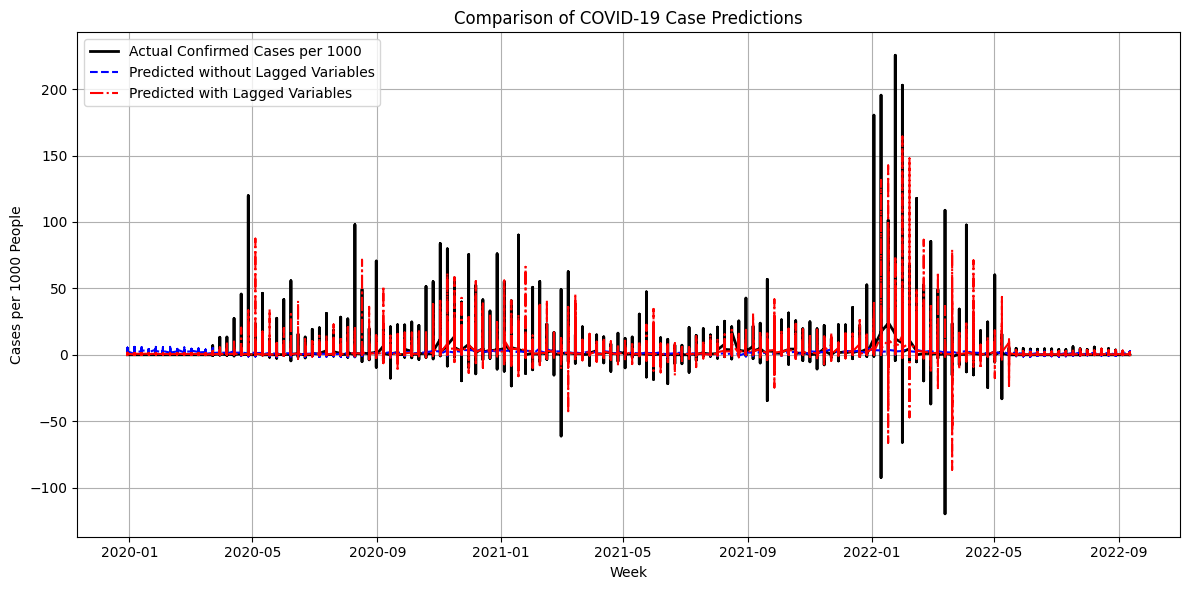
\includegraphics[width=\linewidth]{Figures/Enhanced_Regression_Model_Comparison.PNG}
  \caption{Comparative visualization of regression model predictions with and without lagged variables, demonstrating the significant improvement in predictive accuracy with the inclusion of temporal dynamics.}
  \label{fig:regression_model_comparison}
\end{figure}





\subsection{Impact of vaccination on COVID-19 fatality rates} \label{vaccines}

This part of the study explores the impact of vaccination rates on COVID-19 fatality rates using classification decision trees. Two primary feature variables were selected for analysis:

\begin{itemize}
\item \textbf{Vaccination Rate:} the ratio of the cumulative number of fully vaccinated individuals to the total population.
\item \textbf{Old Population Rate:} the sum of the population percentages between the ages of 50 and 69 relative to the total population.
\end{itemize}

The target variable considered in this analysis is the Death Rate, which is calculated by dividing the total confirmed deaths by the population. The Death Rate is transformed into a binary variable. Death rates exceeding the median value across the dataset are labeled as "high," while those below the median are labeled "low."

To ensure stable analysis, small rates were excluded such as records with a death rate less than $1 \times 10^{-7}$ and a confirmed case rate less than $1 \times 10^{-6}$ were removed from the dataset.


The \textit{DecisionTreeClassifier} from \textit{Scikit-learn} was used to build the decision tree model. To prepare for model training and evaluation, the data was split into a training set and a testing set, with 30 \% of the data used for testing to ensure the model's performance can be adequately assessed. The split was performed using a default random seed of 42.

Then a decision tree classifier was trained using the training data. The complexity of the tree was controlled by limiting its depth to three levels. After training, the model was used to predict the outcomes in the test set. The Gini index was chosen as the performance metric as it measures the probability that a randomly selected instance will be incorrectly classified. A lower Gini index indicates a reduced likelihood of misclassification, which means better model performance.

The visual representation of the result of the decision tree is shown in Figure \ref{fig:decision-tree}. Performance metrics of the classification are summarized in Table \ref{Table:Corr-results}. The decision tree visualization shows the classification based on vaccination rates and the proportion of the older population to predict high or low COVID-19 death rates. First, we observe the root node splits the dataset based on the vaccination rate. This suggests an initial significant relationship between the vaccination rate and death rates. Other splits are using older population rate thresholds which show that higher vaccination rates generally correspond to lower death rates in regions with higher older population rate. In addition, in branches where the old population is high and vaccination rate is low, the classification shows a higher death rate.

As summarized in Table \ref{Table:Corr-results}, the model accuracy is a bit over 65 \%, suggesting that the model has a reasonable degree for predection. In addition, the accuracy is balanced between the two classes. Future work should focus on improving the accuracy of the classification model.

In conclusion, the decision tree classification shows that an increased vaccination rate in counties with higher older population rates decreases the mortality rate in the county. This shows correlation between vaccine and and lowe mortality rate for older population. 

\begin{table}[h]
\centering
\caption{Classification Metrics}
\begin{tabular}{|c|c|c|c|c|}
\hline
\textbf{Class} & \textbf{Precision} & \textbf{Recall} & \textbf{F1-score} & \textbf{Support} \\ \hline
0              & 0.65               & 0.70            & 0.67              & 22305            \\ \hline
1              & 0.66               & 0.61            & 0.63              & 21670            \\ \hline
\multicolumn{5}{|c|}{\textbf{Accuracy: 0.6523 (43975 instances)}}                         \\ \hline
\multicolumn{5}{|c|}{\textbf{Macro Avg:} Precision: 0.65, Recall: 0.65, F1-score: 0.65}  \\ \hline
\multicolumn{5}{|c|}{\textbf{Weighted Avg:} Precision: 0.65, Recall: 0.65, F1-score: 0.65} \\ \hline
\end{tabular}
\label{Table:Corr-results}
\end{table}


\begin{figure*}[h]
  \centering
  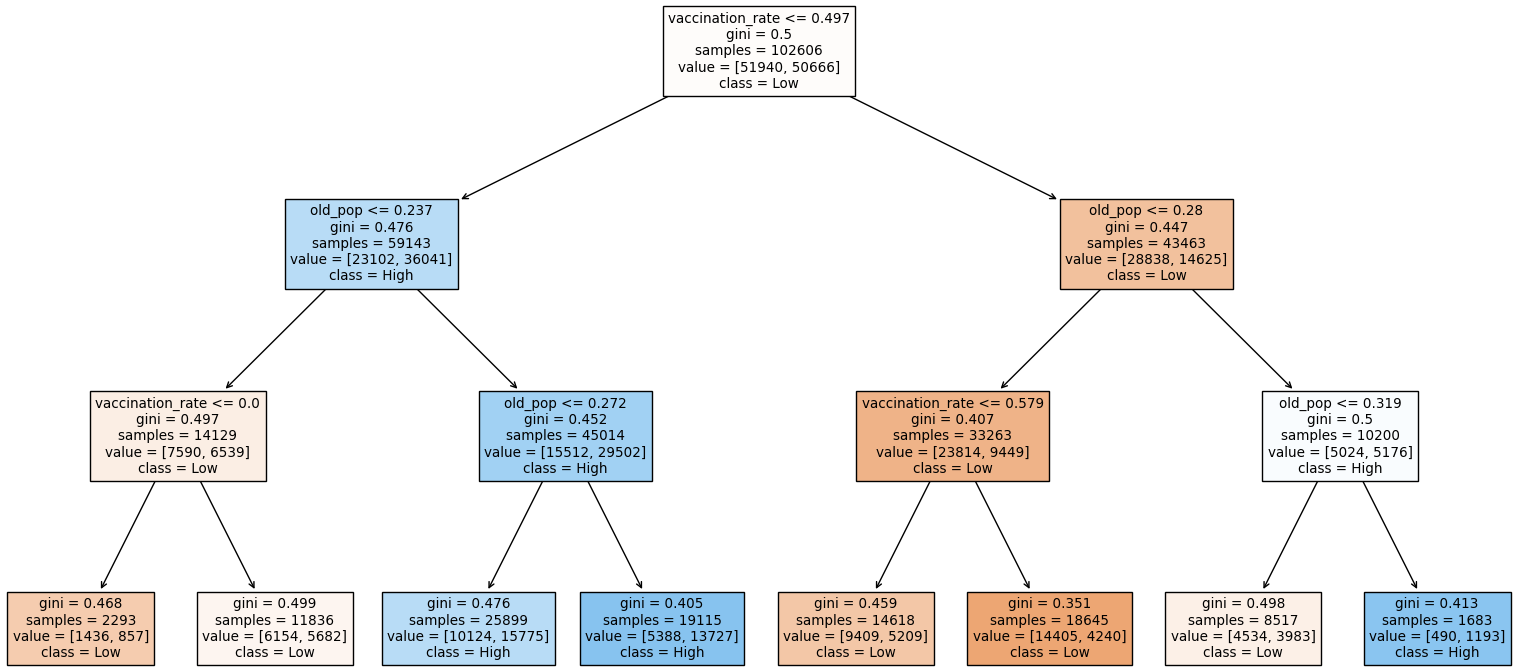
\includegraphics[width=\linewidth]{Figures/tree_high_res.png}
  \caption{Classification tree, where the target variable is the death rate is High or low compared to the median.}
  \Description{Classification tree}
  \label{fig:decision-tree}
\end{figure*}


\subsection{Impact of weather on COVID-19 rates} \label{weather-clustering}

The K-means clustering algorithm from the \texttt{sklearn} library was used to find the relationship between the weather conditions and the COVID-19 infection rates by analyzing three-dimensional data on average daily temperature, relative humidity, and confirmed cases per capita. Data with confirmed case rates lower than 0.01\% were removed to simplify the detection. 



Four different clusters are selected for the analysis based on Inertia sensitivity analysis shown in Figure \ref{fig:Intertia}. Inertia measures the distance between each data point and its centroid, which quantifies the performance of the cluster. Standard scaler was used to scale the data as the attributes have different dimensions. The standard score of a sample x is calculated as:

\begin{equation}
z = (x - u) / s
\end{equation}

\noindent where u is the mean of the data, and s is the standard deviation

\begin{figure}[H]
  \centering
  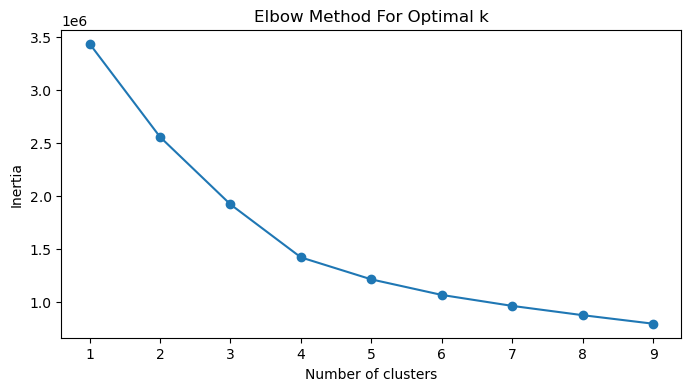
\includegraphics[width=\linewidth]{Figures/Interia.png}
  \caption{Inertia for different number of clusters.}
  \Description{Inertia}
  \label{fig:Intertia}
\end{figure}

The resulting three-dimensional cluster visualization is displayed in Figure \ref{fig:3D-Cluster}. It is observable that cluster 3 is superimposed above clusters 0, 1 and 2, which indicates a higher incidence of confirmed cases within cluster 3. As shown in Figure \ref{fig:confirmedPerCluster}, cluster 3 confirmed cases rates are much higher than other clusters. 

\begin{figure}[H]
  \centering
  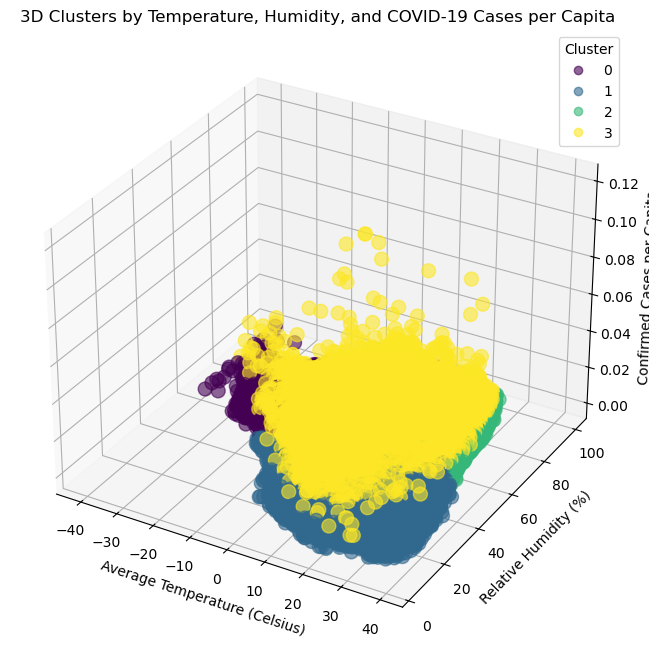
\includegraphics[width=\linewidth]{Figures/3DClusters.PNG}
  \caption{Scatter plot COVID-19 Cases per Capita, Temperature and Humidity colored by cluster number.}
  \Description{Scatter Plot}
  \label{fig:3D-Cluster}
\end{figure}

\begin{figure}[H]
  \centering
  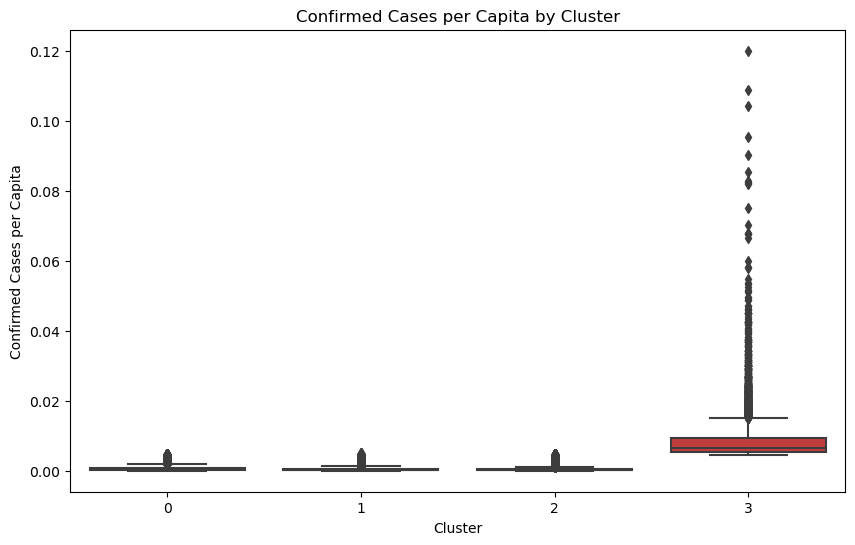
\includegraphics[width=\linewidth]{Figures/confirmedPerCluster.png}
  \caption{Box plot for the different clusters.}
  \Description{Scatter plot COVID-19 Cases per Capita, Temperature and Humidity colored by cluster number }
  \label{fig:confirmedPerCluster}
\end{figure}


A two-dimensional projection, illustrating temperature and humidity within cluster 3, is presented in Figure \ref{fig:2D-cluster}. The data has a temperature range of -30\textdegree{}C to 30\textdegree{}C and humidity levels above 20\%. 

This analysis shows a decrease in the transmissibility of COVID-19 at temperatures exceeding 30\textdegree{}C, under 30\textdegree{}C, or under a 20\% relative humidity.



\begin{figure}[H]
  \centering
  \includegraphics[width=\linewidth]{Figures/Cluster3-2D.PNG}
  \caption{Temperature and humidity 2D projection of cluster 3.}
  \Description{2D projection of cluster 3.}
  \label{fig:2D-cluster}
\end{figure}

\subsection{Preliminary plots}
\begin{figure}[H]
  \centering
  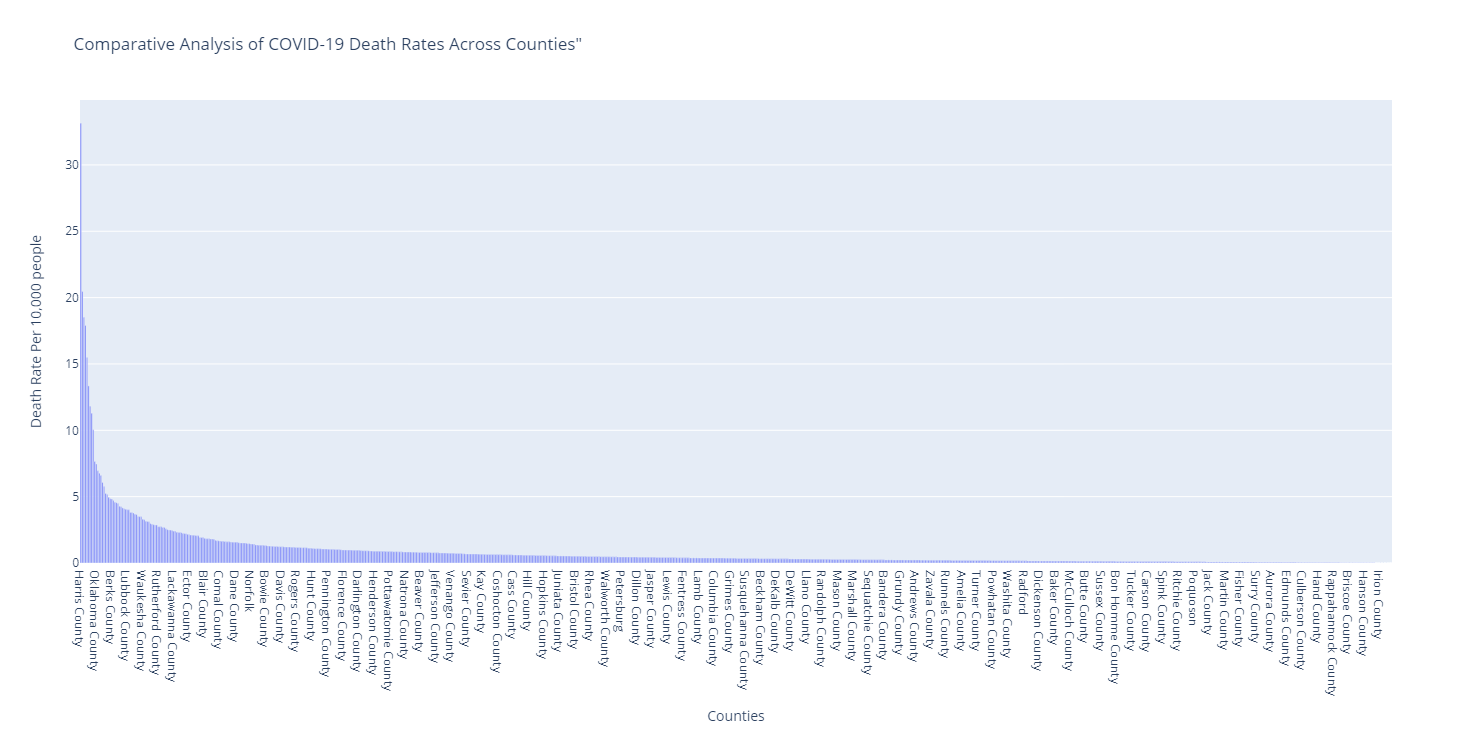
\includegraphics[width=\linewidth]{Figures/3daymovingaverage.png}
  \caption{County-Level 3-Day Moving Average of COVID-19 Mortality Rates Per 10,000 Residents}
  \Description{This figure displays the smoothed mortality rates across various counties, highlighting regions with the highest deaths using a 3-day moving average approach.}
  \label{fig:3day_moving_average_mortality}
\end{figure}

As illustrated in the figure above, Harris County emerges as an outlier among the other counties. While the visualization initially appears static, utilizing Plotly Express enables dynamic exploration through panning and zooming. This capability reveals counties that may not be immediately visible. This analytical approach was employed to identify which counties were most severely impacted
\begin{figure}[H]
  \centering
  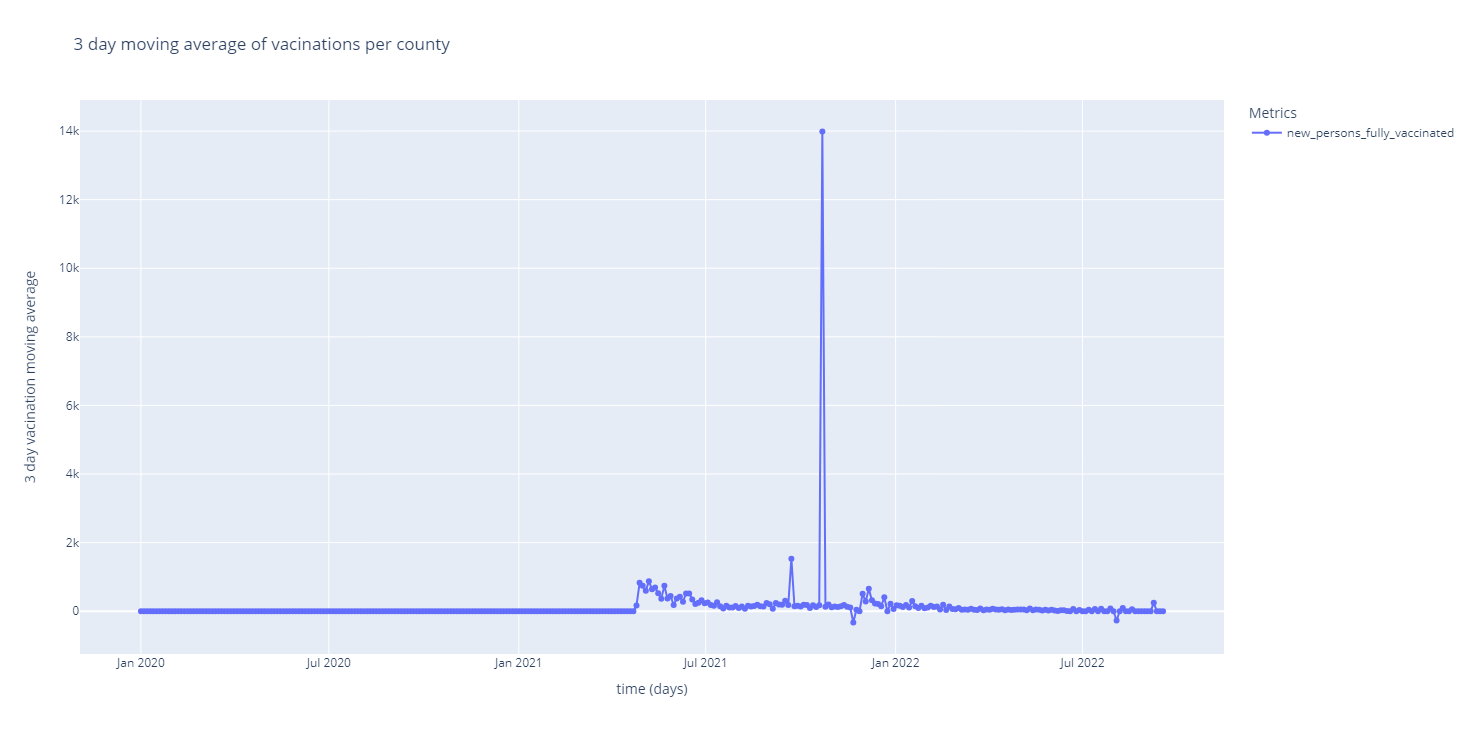
\includegraphics[width=\linewidth]{Figures/3daymovingaveragevacines.png}
  \caption{County-Level 3-Day Moving Average of Daily Vaccinations}
  \Description{This figure illustrates the average daily vaccinations over a 3-day period, providing insights into the vaccination trends across counties.}
  \label{fig:3day_moving_average_vaccines}
\end{figure}
\noindent
The plot shown in figure 14 illustrates a significant spike in COVID-19 vaccination rates from July 2021 to January 2022, a pivotal period in the global vaccination campaign. This rise coincides with the widespread availability of vaccines and concerted efforts by governments and health organizations to increase vaccine uptake amidst the threat of emerging variants.

\begin{figure}[H]
  \centering
  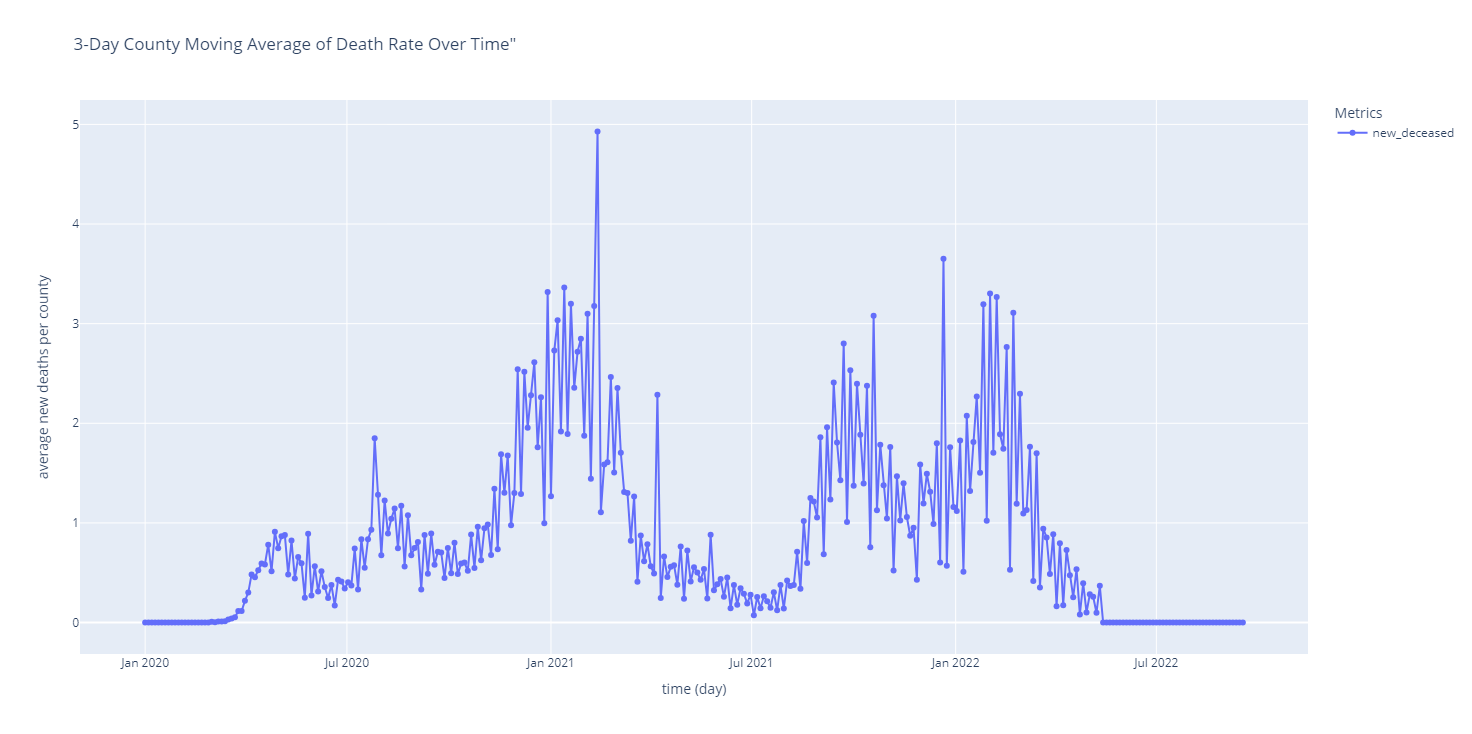
\includegraphics[width=\linewidth]{Figures/Temporal3daymovingaverageDeaths.png}
  \caption{Temporal Analysis of 3-Day Moving Average Deaths at the County Level}
  \Description{This figure tracks the 3-day moving average of deaths over time, revealing temporal trends and patterns in mortality at the county level.}
  \label{fig:temporal_3day_moving_average_deaths}
\end{figure}
\noindent
The plot reveals two peak outbreaks, mirroring the events reported in the news at the time. This correspondence serves as a form of validation for our data, confirming its accuracy with the observed real-world events.
\subsection{Moving Geo-spatial plot}
After compiling the CSV files from a 17-day period and utilizing our binning method to create visual representations, we were able to observe the progression of COVID-19 dynamically. The observed trends closely matched the waves shown in Figure 15 of the temporal chart, offering a clear visualization of the pandemic's development during this interval. Furthermore, the dynamic visuals revealed that regions experiencing outbreaks often influenced nearby areas, suggesting a regional spread. The video illustrating this plotting method can be found at the following link: https://youtu.be/2a9N2mA-I6k


\section{Applications}


\subsection{Impact of COVID-19 mobility}
The data confirm the relationship between increased COVID-19 cases and reduced mobility in workplaces and transit centers. However, the data also indicate increased residential mobility correlating with rising COVID-19 rates. Careful consideration should be given to the fact that closures of outdoor venues may lead to increased indoor mobility when imposing future restrictions.



\subsection{Vaccines impact on death rates}
The analysis shows a relationship between increasing vaccination rates and decreasing death rates in populations over 50 years old. The analysis supports the hypothesis that vaccination reduces mortality across the entire population. However, enforcing vaccinations remains a controversial topic.


\subsection{Weather and COVID-19 Rates}
This study shows a decrease in the transmissibility of COVID-19 at temperatures exceeding 30\textdegree{} C, below 30\textdegree{} C, or under 20\% relative humidity. The reason for this decrease is not identified within the scope of this study. It could be due to reduced virus transmissibility in extreme weather conditions or decreased mobility in such conditions. This information could be used to adjust pandemic restrictions during extreme weather.

\subsection{Geospatial Applications}
The geospatial analysis confirms that when a county is experiencing a significant surge in cases relative to the rest of the country, there is a tendency that nearby and neighboring counties will experience an outbreak simultaneously or shortly after. Also, if several counties are experiencing a significant outbreak in a region, then the counties between the worst counties will also experience an uptick in cases and deaths. This confirms the intuition that COVID-19 will spread indiscriminately from county to county, and counties should prepare for significant COVID-19 exposure if nearby areas of the country are having an outbreak.

\section{Constraints on Data-Driven Analyses}

\subsection{Male and Female attribute}
Initially, we aimed to explore how COVID death rates were influenced by sex. When the data was first extracted, we observed that some counties included columns for males and females, prompting us to consider this attribute in our analysis. Upon further exploration, however, we discovered that these values merely represented the total populations of males and females in each county, not the specific numbers who contracted COVID or died from it. This discrepancy meant that we could not include sex as a factor in our analysis.

\subsection{Mobility}
Additionally, we identified a "mobility" value in the dataset, initially presumed to reflect travel frequency. However, upon further analysis, the exact nature of this attribute remained unclear. To maintain the integrity of our analysis, we chose not to include it without a clear understanding of what it represented.

\subsection{Reporting Variance}
Due to the nature of the COVID-19 Open Data by Google, data granularity at the county and state levels was reported differently depending on the county or state. Some states, for example, reported certain search terms for symptoms that others did not. It was unclear if the absence of those search terms from any given county meant that the term was not searched for or if that term was not reported for another reason. Many search terms were entirely missing from the majority of counties, but the explanation for the absence was unknown. As such, it became impractical to perform frequent set analysis or to fill in missing data using any of the rules discussed in class.



\section{Comparison with Published Results}
Our data yield the similar conclusion to data that has already been done on COVID. We from temporal chart analysis that COVID seems to have a spike in rates during winter. Additionally there were also two big waves of data which can be seen in both the temporal charts and the Geo-spatial charts plotted with respect to time.






\newpage
%%
%% The next two lines define the bibliography style to be used, and
%% the bibliography file.
\bibliographystyle{ACM-Reference-Format}
\bibliography{sample-base}


\end{document}
\endinput
%%
%% End of file `sample-sigconf.tex'.
